\documentclass[pdflatex,sn-basic]{sn-jnl}
\usepackage{amsmath,amssymb,booktabs,graphicx,algorithm,algpseudocode}
\theoremstyle{thmstyleone}\newtheorem{proposition}{Proposition}\newtheorem{theorem}{Theorem}
\theoremstyle{thmstylethree}\newtheorem{remark}{Remark}
\raggedbottom
\usepackage{array}\newcolumntype{L}[1]{>{\raggedright\arraybackslash}p{#1}}
\newcommand{\hd}[1]{\begin{tabular}[b]{@{}c@{}}#1\end{tabular}}
\begin{document}
\title[Revealed Aspiration Levels]{Revealed Aspiration Levels: Inverse Interval Goal Programming for Recovering the Targets and Priorities Behind Public Decisions}
\author*[1]{\fnm{Quang-Vinh} \sur{Dang}}\email{vinh.dq4@buv.edu.vn}
\affil*[1]{\orgname{British University Vietnam}, \orgaddress{\city{Hung Yen}, \country{Vietnam}}}
\abstract{Governments, central banks and firms announce targets, but what they pursue can only be read from what they do. We formulate the recovery of aspiration levels from sequential decisions as an inverse interval goal program with asymmetric weights and an adjustment cost; a change of variables makes the optimality conditions linear in the unknowns. Aspiration levels are revealed when a decision stops at a band edge; weights are not point-identified under a linear adjustment cost but are under a quadratic one, given a rank condition and the other parameters. For one goal we give the optimal policy in closed form, an exact polynomial-time estimator and a consistency result; for several goals, a mixed-integer formulation and a multistart heuristic. Implied inflation targets of fourteen central banks have the right magnitude but are no closer to stated targets than a constant 2.5\%. Among 23 aid donors, a combined test with multiplicity adjustment finds nonlinear state dependence inconsistent with partial adjustment for one to three donors; among them Sweden and Norway reveal targets of 0.90 and 0.98\% of GNI, near their national 1\% goals, while most EU donors reveal targets well below their 0.7\% commitment. NATO allies' revealed lower edge rose from about 2\% to 3.2\% of GDP after 2022, a shift the bootstrap separates but the profile loss does not; no test distinguishes defence decisions from simpler behaviour. A one-goal model is uninformative for corporate leverage, and the goal program does not predict decisions better than simple rules; its use is in reading aspiration levels.}
\keywords{Goal programming, Inverse optimization, Aspiration levels, Revealed preferences, Mixed-integer programming, Public budgets}
\maketitle
\section{Introduction}
Goal programming (GP) asks a decision maker for aspiration levels and priorities and returns a decision \citep{charnes1961,tamiz1998}. Many public and corporate actors announce aspiration levels (an inflation target, a defence spending guideline, an aid commitment, a leverage policy) and then decide repeatedly. The inverse question is natural and practically important: given the observed decisions, which aspiration levels and priorities would make them optimal? Comparing revealed with stated aspirations measures credibility; tracking them over time shows when priorities change.

Related questions have been studied in inverse optimization, which recovers parameters that make observed solutions optimal \citep{ahuja2001,chan2025review}, and in economics, where implicit inflation targets of central banks and welfare weights of governments are estimated from policy \citep{dennis2006,hendren2020}. Section~\ref{sec:lit} reviews both. Asymmetric and zone-like preferences of central banks are also estimated in monetary economics \citep{orphanides2002,rugemurcia2003,kilian2008}, and online and contextual inverse optimization learn objectives from streams of decisions \citep{besbes2025}. We did not find a method that recovers the aspiration bands of goal programs from noisy sequential decisions with an exact estimator and conditions for identification.

\paragraph{Contributions.} (i) A forward model for repeated decisions under interval goals with an adjustment cost, and a change of variables that makes the inverse problem linear apart from discrete states (Section~\ref{sec:model}). (ii) Structural results: breakpoint optimality, effective weights, exact revelation of aspiration levels at band edges, non-identifiability of weights under linear adjustment cost and a rank condition for their point identification under quadratic adjustment cost (Section~\ref{sec:ident}). (iii) Estimation: a closed-form policy and an exact polynomial-time algorithm with a certified optimality gap for one goal, an exact MILP for several goals, and a scalable multistart heuristic (Section~\ref{sec:alg}); and a consistency theorem for the decision-space estimator (Section~\ref{sec:consistency}). The guarantees are strongest for one goal, where all parameters are identified and the estimator is exact and consistent; for several goals, weights are identified when the other parameters are known, the MILP solves only small instances to optimality, and the multistart heuristic carries no guarantee. All applications except central banks use one goal. (iv) Applications to four kinds of decision makers (Section~\ref{sec:apps}): central banks, whose public targets allow a pre-specified check, aid donors, defence ministries and listed firms; and a study of model adequacy with placebo experiments, tests of state dependence and of partial adjustment, and out-of-sample comparisons (Section~\ref{sec:adequacy}).

\subsection{Related literature}\label{sec:lit}
\paragraph{Goal programming.} Goal programming minimises unwanted deviations from aspiration levels \citep{charnes1961,charnes1977}, a term that goes back to Simon's satisficing decision maker, who stops searching once an aspiration level is met \citep{simon1955}; its weighted, lexicographic and Chebyshev variants, interval goals and the elicitation of aspiration levels are surveyed by \citet{tamiz1998}. Extensions to uncertainty (stochastic, fuzzy and robust goal programming) take the parameter distribution or uncertainty set as given and change the forward problem. Our question is different: the aspiration levels and priorities are the unknowns, and the data are the decisions they produce.

\paragraph{Inverse optimization.} Inverse optimization recovers parameters that make observed solutions optimal \citep{ahuja2001}; \citet{chan2025review} review theory and applications. With many noisy observations, \citet{keshavarz2011} impute convex objectives by minimising residuals of optimality conditions, \citet{bertsimas2015} estimate equilibria, and \citet{aswani2018} show that estimators based on optimality conditions can be inconsistent while the decision-space loss is consistent but hard to compute. Distributionally robust and regret-based formulations \citep{esfahani2018,besbes2025} and the incenter and augmented suboptimality loss of \citet{zattoni2025} address noise and non-uniqueness. For linear programs the cost vector is generically not point-identified \citep{ahmadi2026}. We use the decision-space loss, and the goal-programming structure gives what general methods lack here: a closed-form policy for one goal, an exact polynomial-time estimator, and explicit conditions under which aspiration levels and weights are identified.

\paragraph{Inverse multiobjective optimization and inverse goal programming.} \citet{chan2014} infer objective weights of a multiobjective radiation-therapy plan and show that weights are unique only when the observed point lies in the relative interior of a facet; \citet{chanlee2018} preserve trade-offs, \citet{dongzeng2021} add distributional robustness, \citet{gebken2021} infer criteria from data, and \citet{carrizosa2026} cluster decision makers by inferred preferences under linear objectives. These works infer weights; aspiration levels, which define goal programs, are not inferred. The only paper we found under the name inverse goal programming adjusts deviation weights so that a single noiseless solution becomes optimal with targets fixed \citep{saif2023}.

\paragraph{Inverse reinforcement learning.} Inverse reinforcement learning and inverse optimal control recover the reward of a sequential decision maker from demonstrated behaviour \citep{ng2000,ziebart2008}. They allow general rewards and dynamics but give no closed-form policy, exact estimator or identification result for the goal-programming structure; our forward model is myopic, which is what makes those results possible.

\paragraph{Learning and optimisation.} Predict-then-optimise and decision-focused learning train predictors for a downstream optimisation problem \citep{elmachtoub2022,hu2022,mandi2024}, including goal-based investment problems solved by goal programming \citep{bae2026}. There, the optimisation model is given and its inputs are learned; here, the decisions are given and the optimisation model is learned.

\paragraph{Revealed preferences of public actors.} The term ``revealed'' follows revealed-preference theory, which tests and recovers preferences from observed choices \citep{afriat1967,varian1982}. Economists recover preference parameters from policy: inequality aversion from the allocation of public services \citep{behrman1987}, and social welfare weights from tax schedules by inverting optimal-tax conditions \citep{bourguignon2012,saez2016,hendren2020,lockwood2016}. For central banks, implicit inflation targets and loss weights are estimated from interest-rate decisions with quadratic losses or policy rules \citep{taylor1993,clarida2000,svensson1997,dennis2006,favero2003,ozlale2003,ireland2007}, and \citet{shapiro2021} estimate asymmetric piecewise-linear losses from text, which in our terms is a one-goal interval goal program. A closely related line studies asymmetric and zone-like central-bank preferences: the opportunistic approach to disinflation, in which policy acts only when inflation leaves a range \citep{orphanides2002}, and estimates of asymmetric preference parameters from policy rules and inflation outcomes \citep{rugemurcia2003,surico2007,kilian2008}. These papers specify a loss for one policy maker and estimate its parameters by regression or moment conditions; the policy shape we derive (inaction inside a band, partial correction outside it, bounded steps) has the same economic content, and our contribution for this case is the exact estimator and its identification analysis. For aid, allocation regressions relate flows to recipient need and donor interests \citep{alesina2000}, and a recent working paper applies inverse optimization to donors' weights on need, alignment and commerce \citep{karamifard2026}. For firms, partial adjustment towards a target capital structure \citep{flannery2006} is the empirical counterpart of gradual adjustment. Relative to this literature, the goal-programming formulation makes aspiration bands and asymmetric step sizes explicit parameters, allows several goals, and reports sets when the data do not determine a point.

\section{Model and identification}\label{sec:modelident}
\subsection{Forward model}\label{sec:model}
At decision time $t$ the decision maker observes $x_t\in\mathbb{R}^K$, the values goal variables would take if the policy were unchanged, and chooses a change $D$. Goal $k$ responds linearly, $y_k(D)=x_{kt}+\beta_k D$ with $\beta_k\neq 0$. Each goal is an interval goal $[\tau_k-b_k,\tau_k+b_k]$ with weights $w_k^+$ for overshooting and $w_k^-$ for undershooting. With adjustment cost $C(D)$,
\begin{equation}\label{eq:forward}
F_t(D)=\sum_{k=1}^K\Big[w_k^+\big(y_k(D)-\tau_k-b_k\big)_+ + w_k^-\big(\tau_k-b_k-y_k(D)\big)_+\Big]+\lambda\,C(D).
\end{equation}
We study $C(D)=|D|$ (linear) and $C(D)=D^2/2$ (quadratic), and normalise $\lambda=1$ (Proposition~\ref{prop:eff}). Gradual adjustment of this kind is the behaviour of central banks that change rates in repeated small steps and of firms that adjust leverage partially towards a target \citep{flannery2006}. For $\beta_k<0$ let $\alpha_k=1/|\beta_k|$, $c_k=\alpha_k\tau_k$, $d_k=\alpha_k b_k$, $\omega_k^\pm=w_k^\pm/\alpha_k$ and $g_{kt}(D)=\alpha_k x_{kt}-D-c_k$. Then
\begin{equation}\label{eq:scaled}
F_t(D)=\sum_k\Big[\omega_k^+\big(g_{kt}(D)-d_k\big)_+ + \omega_k^-\big(-g_{kt}(D)-d_k\big)_+\Big]+\lambda\,C(D),
\end{equation}
in which, for given discrete states (which goals are above, on, inside or below their bands), the kinks are linear in $(\alpha,c,d,D)$ and the slopes are the weights. For controls that move the goal variable one-for-one (budget shares), the decision is the change $\Delta$ of the share; writing $D=-\Delta$ gives $\beta=-1$ and $\alpha=1$, so $D>0$ is a cut. Table~\ref{tab:notation} summarises the notation.
\begin{table}[t]\centering\small
\begin{tabular}{L{0.36\textwidth}L{0.56\textwidth}}\toprule
Symbol & Meaning\\\midrule
$x_{kt}$ & value of goal variable $k$ at time $t$ if policy is unchanged (the state)\\
$D_t$, $\Delta_t$ & decision (change of the instrument); $\Delta=-D$ for one-for-one controls\\
$\beta_k$, $\alpha_k=1/|\beta_k|$ & transmission of the decision to goal $k$, and its inverse\\
$\tau_k$, $b_k$ & aspiration level and half-width of the tolerance band $[\tau_k-b_k,\tau_k+b_k]$\\
$w_k^\pm$, $\omega_k^\pm=w_k^\pm/\alpha_k$ & deviation weights and effective weights (step sizes under quadratic cost)\\
$c_k=\alpha_k\tau_k$, $d_k=\alpha_kb_k$, $e_k^\pm=c_k\pm d_k$ & transformed aspiration level, half-width and band edges\\
$Q_T(\theta)$ & decision-space loss $\frac1T\sum_t|D_t-D_t^*(\theta)|$\\
\bottomrule\end{tabular}
\caption{Notation.}\label{tab:notation}\end{table}

\subsection{Identification}\label{sec:ident}
Throughout, $w_k^\pm\ge0$, $b_k\ge0$, the adjustment-cost weight is normalised to $\lambda=1$, and every observed decision is assumed to be a strict minimiser of $F_t$ (for the quadratic cost this holds automatically; for the linear cost it is the strict-optimality margin used in estimation).

\begin{proposition}[Breakpoints]\label{prop:bp}
Let $C(D)=|D|$. Then $F_t$ is convex and piecewise linear with $F_t(D)\ge|D|$, so it attains its minimum, and every strict minimiser lies in $\mathcal{C}_t=\{0\}\cup\{D: x_{kt}+\beta_kD=\tau_k\pm b_k,\ k=1,\dots,K\}$. When all $\beta_k<0$, $\mathcal{C}_t=\{0\}\cup\{\alpha_kx_{kt}-c_k\mp d_k\}_k$.
\end{proposition}
\begin{proof}
Each term is convex and piecewise linear in $D$, and the goal terms are nonnegative, so $F_t\ge|D|$ and $F_t$ is coercive; it attains its minimum. A convex piecewise-linear function is affine between consecutive kinks; a strict minimiser cannot lie in the interior of an affine piece, so it is a kink. The kinks are $D=0$ (from $|D|$) and the points where some goal variable reaches a band edge.
\end{proof}

\begin{proposition}[Normalisation and effective weights]\label{prop:eff}
Decisions are invariant to scaling $(w,\lambda)\mapsto\kappa(w,\lambda)$, $\kappa>0$, which is why $\lambda=1$. Given the sign of each $\beta_k$, the map $(w_k,\beta_k)\mapsto(\alpha_k,\omega_k)$ with $\alpha_k=1/|\beta_k|$, $\omega_k=w_k|\beta_k|$ is a bijection, so $w_k=\alpha_k\omega_k$ is identified whenever $\alpha_k$ and $\omega_k$ are. Decisions depend on the weights only through $\omega$, the marginal goal gain per unit of policy, which is the natural object for estimation.
\end{proposition}
\begin{proof}
Both claims follow from \eqref{eq:scaled}.
\end{proof}

\begin{proposition}[Edge revelation]\label{prop:edge}
Let $\beta_k<0$. If in period $t$ the strict minimiser lies on the upper (lower) band edge of goal $k$, then $\tau_k+b_k=x_{kt}-D^*_t/\alpha_k$ (respectively $\tau_k-b_k$). Hence, if the binding goal and edge are known for two upper-edge periods of goal $k$ with distinct $x_{kt}$ and one lower-edge period, then $\alpha_k$, $\tau_k$ and $b_k$ are determined.
\end{proposition}
\begin{proof}
On the upper edge $D^*_t=\alpha_kx_{kt}-(c_k+d_k)$, a linear equation in $(\alpha_k,c_k+d_k)$; two such equations with distinct $x_{kt}$ determine both. A lower-edge period then gives $c_k-d_k=\alpha_kx_{kt}-D^*_t$, hence $c_k$, $d_k$, $\tau_k=c_k/\alpha_k$ and $b_k=d_k/\alpha_k$.
\end{proof}
The condition is sufficient, not necessary, and the binding goal and edge of a period are latent in practice; the estimator in Section~\ref{sec:alg} treats them as discrete states.

\begin{proposition}[Weights are not point-identified under linear cost]\label{prop:set}
Let $C(D)=|D|$ and fix $(\alpha,c,d)$. The set of weights $\omega\ge0$ under which every observed decision is a strict minimiser is defined by finitely many strict linear inequalities. If it is nonempty it is relatively open in the nonnegative orthant and has full dimension, so it is not a single point and the weights are not point-identified. Jointly over $(\alpha,c,d,\omega)$ the identified set is a finite union of such sets and need not be convex.
\end{proposition}
\begin{proof}
For fixed $(\alpha,c,d)$ the state of each goal at $D^*_t$ (strictly above, on the edge, strictly inside, strictly below) is fixed, and the one-sided derivatives of $F_t$ at $D^*_t$ are affine in $\omega$ with coefficients determined by these states. Strict optimality is right derivative $>0$ and left derivative $<0$ in every period: finitely many strict linear inequalities, whose solution set $U$ is open. If $p\in U\cap\{\omega\ge0\}$, a ball around $p$ lies in $U$, and its intersection with the orthant has nonempty interior because $p$ belongs to the orthant, which is convex and full-dimensional. Varying $(\alpha,c,d)$ changes the states only at finitely many hyperplanes, which gives the finite union. The result relies on strict optimality; with weak optimality the set is closed and can degenerate to a point, so it describes the generic case. With noisy decisions its counterpart is the non-uniqueness of the population minimiser (Theorem~\ref{thm:misspec}). For one goal the set is, in the region where the goal is outside its band, a half-line in each weight: what is not identified is the scale of the weights relative to the linear adjustment cost, which is normalised to one.
\end{proof}

\begin{proposition}[Weights under gradualism]\label{prop:quad}
Let $C(D)=D^2/2$ and $\beta_k<0$ for all $k$. Then $F_t$ is $1$-strongly convex, its minimiser $D^*_t$ is unique and continuous in the parameters, and $D^*_t=\sum_{k\in A_t}\omega_k^+-\sum_{k\in B_t}\omega_k^-+\sum_k\pi_{kt}$, where $A_t$ ($B_t$) is the set of goals strictly above (below) their bands at $D^*_t$ and $\pi_{kt}$ are multipliers of goals sitting exactly on an edge. In particular, if at $D^*_t$ exactly one goal $k$ is strictly above its band and every other goal is strictly inside its band, then $\omega_k^+=D^*_t$; if exactly one goal is strictly below, $\omega_k^-=-D^*_t$. If $(\alpha,c,d)$ are known, so that the sets $A_t$ and $B_t$ are known, the weights are point-identified if the incidence matrix of $(A_t,B_t)$ over the periods in which no goal sits on an edge has full column rank.
\end{proposition}
\begin{proof}
$F_t-D^2/2$ is convex, so $F_t$ is $1$-strongly convex in $D$ uniformly in the parameters, and it is Lipschitz in the parameters on bounded sets; hence the minimiser is unique and continuous. Stationarity $0\in\partial F_t(D^*_t)$ gives the expression, with $p_k=\omega_k^+$ for goals strictly above, $q_k=\omega_k^-$ for goals strictly below, zero for goals strictly inside, and a multiplier in an interval for goals on an edge. In periods without edge goals the equations $D^*_t=\sum_{A_t}\omega_k^+-\sum_{B_t}\omega_k^-$ are linear in $\omega$ with incidence coefficients $\pm1$, and a linear system whose matrix has full column rank has at most one solution. The condition is sufficient, not necessary: periods with goals on an edge add the inequalities $0\le\pi_{kt}\le\omega_k^\pm$, which can also restrict the weights.
\end{proof}
\begin{remark}
Under gradualism, while a single goal is outside its band and the others are inside, the decision maker moves by the constant step $\omega_k^\pm$ when the goal is more than one step from the band edge, and otherwise moves exactly to the edge and stops (the ramp in Theorem~\ref{thm:closed}). With two goals outside their bands only the sum of their weights is revealed. Proposition~\ref{prop:quad} takes $(\alpha,c,d)$ as known; joint identification of aspiration levels and weights is proved for one goal in Theorem~\ref{thm:cons} and remains open for several goals. Two interpretations of $\omega$ are observationally equivalent: a goal weight relative to a quadratic adjustment cost, and a cap on the size of each step (a rate limit); a decision maker who moves towards a target by at most a fixed amount per period produces the same decisions (Theorem~\ref{thm:closed}); the rate-limited quadratic program in the placebo experiments of Section~\ref{sec:adequacy} is an example. We therefore call $\omega^\pm$ step sizes and read them as revealed priorities only under the goal-programming interpretation. For controls that move a share one-for-one ($\alpha=1$, $D$ replaced by $-D$), $\omega^+$ is the size of a cut when the share is above its band and $\omega^-$ the size of an increase when it is below.
\end{remark}

\section{Estimation}\label{sec:alg}
Observed decisions are $D_t=D_t^*+\varepsilon_t$. We minimise the decision-space loss $Q_T(\theta)=\frac1T\sum_t|D_t-D^*_t(\theta)|$ over $\theta=(\alpha,c,d,\omega^+,\omega^-)$, which is consistent under standard conditions but hard in general \citep{aswani2018}.

\subsection{Several goals: exact formulation and multistart search}\label{sec:multi}
\paragraph{Exact MILP.} For several goals we write the estimator as a mixed-integer linear program. Decision variables are the parameters $(\alpha,c,d,\omega^+,\omega^-)$, fitted decisions $\hat D_t$, residuals $r_t\ge|D_t-\hat D_t|$ (with $D_t$ the observed decisions) and, for each period and goal, binaries $a_{kt}$ (at or above the upper edge, $g_{kt}-d_k\ge0$), $s_{kt}$ (strictly above), $l_{kt}$ (at or below the lower edge) and $z_{kt}$ (strictly below), with $s_{kt}\le a_{kt}$ and $z_{kt}\le l_{kt}$. With $g_{kt}=\alpha_kx_{kt}-\hat D_t-c_k$ linear in the unknowns, big-$M$ constraints link the binaries to the kinks, e.g.\ $g_{kt}-d_k\le Ma_{kt}$, $g_{kt}-d_k\ge-M(1-a_{kt})$, $g_{kt}-d_k\le Ms_{kt}$ and $g_{kt}-d_k\ge\delta-M(1-s_{kt})$. Under quadratic cost, stationarity is $\hat D_t=\sum_k(p_{kt}-q_{kt})$ with multipliers $0\le p_{kt}\le\omega_k^+$, $p_{kt}\le\Omega a_{kt}$ and $p_{kt}\ge\omega_k^+-\Omega(1-s_{kt})$, and similarly for $q_{kt}$. Under linear cost, flat optima would let fitted decisions absorb noise, so we impose a strict-optimality margin $\epsilon$: with binaries $u_t,v_t$ for $\hat D_t>0$ and $\hat D_t<0$, the right derivative $-\sum_k\omega_k^+s_{kt}+\sum_k\omega_k^-l_{kt}+1-2v_t\ge\epsilon$ and the left derivative $-\sum_k\omega_k^+a_{kt}+\sum_k\omega_k^-z_{kt}+2u_t-1\le-\epsilon$, where products of weights and binaries are linearised exactly. The objective is $\frac1T\sum_tr_t$. We use $M=30$ for kinks, $\Omega=5$ for weights and multipliers, $\delta=10^{-3}$ for strict states, $\epsilon=0.05$ for the optimality margin and $\alpha\in[0.05,3]$. The formulation is exact, but it is solved to optimality only for small instances: on our synthetic instances the solver did not close the gap within the time limit (Table~\ref{tab:synth}); for several goals we therefore rely on the heuristic below.


\paragraph{Multistart with exact polishing.} Under quadratic cost the decision loss is continuous in $\theta$, and $D^*_t(\theta)$ is computed exactly by evaluating $F_t$ at the $2K$ breakpoints and at the stationary points of the pieces (our implementation enumerates the $3^K$ possible slope sums; sorting the breakpoints gives $O(K\log K)$). We run Powell's method from many random starts in parallel, then polish the best solutions: with all states fixed the estimation problem is a linear program; large-neighbourhood search frees the states of a subset of periods (largest residuals plus random periods) and solves the small MILP exactly.

\begin{algorithm}[t]\caption{Exact one-goal estimator for fixed $\alpha$ (Theorem~\ref{thm:exact})}\label{alg:exact}
\begin{algorithmic}[1]
\State $z_t\gets\alpha x_t$; $\mathcal{E}\gets\{z_t-D_s\}_{t,s}\cup\{z_t\}_t$, sorted
\For{each $e\in\mathcal{E}$}
  \State $U(e)\gets\min_{\omega\in(\{D_s\}\cup\{z_t-e\})\cap[0,\bar\omega^+]\,\cup\{0\}}\sum_{z_t>e}|D_t-\min(z_t-e,\omega)|$ \Comment{upper part}
  \State $L(e)\gets\min_{\omega\in(\{-D_s\}\cup\{e-z_t\})\cap[0,\bar\omega^-]\,\cup\{0\}}\sum_{z_t<e}|D_t-\max(z_t-e,-\omega)|$ \Comment{lower part}
  \State $A(e)\gets\sum_{z_t\le e}|D_t|$, $B(e)\gets\sum_{z_t<e}|D_t|$ \Comment{prefix sums}
\EndFor
\State return $\min_{e^-\le e^+}\,[L(e^-)-B(e^-)]+[U(e^+)+A(e^+)]$ via a running minimum over sorted $\mathcal{E}$
\end{algorithmic}\end{algorithm}
\begin{algorithm}[t]\caption{Multistart heuristic with exact polishing (several goals)}\label{alg:ms}
\begin{algorithmic}[1]
\For{$j=1,\dots,J$ in parallel} \State $\theta_j\gets$ Powell's method on $Q_T$ from a random start \EndFor
\For{each of the best $m$ solutions $\theta$}
  \State fix the states implied by $\theta$; solve the linear program in $\theta$ (all binaries fixed)
  \For{$i=1,\dots,I$} \State free the states of the $n_{\mathrm{free}}$ periods with largest residuals and random others; solve the sub-MILP; accept if better \EndFor
\EndFor
\State return the best solution
\end{algorithmic}\end{algorithm}

\paragraph{Synthetic evidence.} Table~\ref{tab:synth} summarises runs with $K=2$, $T=80$ and Laplace decision noise. The full MILP stalls on weak relaxations; differential evolution finds the noiseless optimum but not the noisy one; the multistart algorithm reaches a loss below that of the true parameters at noise $0.05$ and recovers aspiration levels, bands, transmission and, approximately, weights; the table reports losses only, and parameter errors over repeated instances are given in the next paragraph.
\paragraph{Repeated recovery.} To see how reliable the multistart algorithm is at the size of the central-bank samples, we drew 20 instances per noise level with $K=2$ and $T=60$ (state 1 an AR(1) around 3, state 2 an AR(1) around 0; true $\alpha=(0.5,1)$, $\tau=(2.5,0)$, $b=(0.5,1)$, $\omega^\pm=(0.5,0.25)$) and fitted each with the default settings used for the banks. The median fitted loss is 5\% below the loss at the true parameters at both noise levels, but the search stops above it in 8 of 20 instances at noise 0.05 and in 5 of 20 at noise 0.10 (at most 31\% above). The median absolute errors for the first goal are 0.02 and 0.09 for $\tau_1$, 0.04 and 0.11 for $b_1$ and 0.03 and 0.14 for $\alpha_1$; the second goal, with a wider band, is recovered less well (median error of $\tau_2$ 0.17 and 0.56). The heuristic therefore recovers a well-informed goal reliably but is not guaranteed to find the global minimum (results/k2\_recovery.csv). On real data we ran the MILP on the shortest bank series (Hungary, $T=33$) for two hours: its best solution has the same loss as the best of five multistart runs (0.2546), but the dual bound is 0.187, a gap of 26.5\%, so even there global optimality is not certified (results/milp\_check\_hu.csv).

\begin{table}[t]\centering\small
\begin{tabular}{llrr}\toprule
Model & Algorithm & \hd{Fitted\\loss} & \hd{Loss at\\true $\theta$}\\\midrule
Linear cost, noise 0.1 & full MILP (120 s) & 0.205 & 0.089\\
 & LNS (29 s) & 0.189 & 0.089\\
 & DE + LP + LNS (32 s) & 0.101 & 0.089\\
Quadratic cost, noise 0 & DE, 3000 generations (189 s) & 0.000 & 0.000\\
Quadratic cost, noise 0.05 & DE + LP + LNS & 0.093 & 0.055\\
 & multistart + LP + LNS (267 s) & 0.052 & 0.055\\
Quadratic cost, noise 0.1 & multistart + LP + LNS (925 s) & 0.111 & 0.106\\
\bottomrule\end{tabular}
\caption{Estimation on synthetic data ($K=2$, $T=80$).}\label{tab:synth}
\end{table}

\subsection{An exact algorithm for one goal}\label{sec:exact}
For a single goal ($K=1$), which covers the budget applications, the estimator can be computed exactly with a certificate. Write $e^\pm=c\pm d$ ($e^-\le e^+$) and $z=\alpha x$.

\begin{theorem}[Closed-form policy]\label{thm:closed}
Let $K=1$, $C(D)=D^2/2$, $\beta<0$, $\omega^\pm\ge0$ and $e^-\le e^+$. Then
\[
D^*(x)=\operatorname{clip}\big(\alpha x-e^+,\,0,\,\omega^+\big)+\operatorname{clip}\big(\alpha x-e^-,\,-\omega^-,\,0\big),
\]
where $\operatorname{clip}(v,a,b)=\min\{\max\{v,a\},b\}$. For direct control of a share ($\alpha=1$, decision $\Delta=-D$), the optimal change is $\Delta^*(x)=-\operatorname{clip}(x-e^+,0,\omega^+)-\operatorname{clip}(x-e^-,-\omega^-,0)$: a cut of at most $\omega^+$ above the band and an increase of at most $\omega^-$ below it.
\end{theorem}
\begin{proof}
Let $u=\alpha x-e^+\le l=\alpha x-e^-$. The goal is above its band for $D<u$, inside for $u<D<l$ and below for $D>l$, so the right derivative of $F$ is $D-\omega^+\mathbb{1}[D<u]+\omega^-\mathbb{1}[D\ge l]$. If $u\ge\omega^+$, the derivative vanishes at $D=\omega^+\le u$; if $0\le u<\omega^+$, it is negative to the left of $u$ and nonnegative to the right, so $D^*=u$; if $u<0<l$, $D^*=0$; the cases $l\le0$ are symmetric. In every case $D^*$ equals the stated expression, whose two terms are never simultaneously nonzero because $u\le l$.
\end{proof}
The policy has a dead zone (no action while the goal is inside the band), ramps of slope $\alpha$ (the decision stops exactly at a band edge) and saturation at the step sizes $\omega^\pm$; because $e^-\le e^+$ it is $1$-Lipschitz in $z$. Figure~\ref{fig:policy} illustrates the shape.
\begin{figure}[t]\centering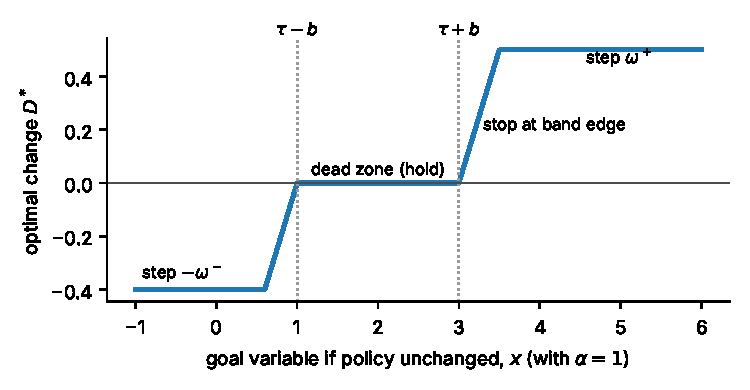
\includegraphics[width=0.75\textwidth]{fig_policy.pdf}
\caption{Optimal policy for one goal under gradualism (Theorem~\ref{thm:closed}), with $\alpha=1$, band $[1,3]$, $\omega^+=0.5$, $\omega^-=0.4$.}\label{fig:policy}\end{figure}

\begin{theorem}[Exact estimation for fixed $\alpha$]\label{thm:exact}
Fix $\alpha$ and optimise over $e^-\le e^+$ and $\omega^\pm\ge0$. The decision-space objective $\sum_t|D_t-D^*(x_t)|$ attains its minimum at a point with $e^\pm\in\mathcal{E}=\{\alpha x_t-D_s\}_{t,s}\cup\{\alpha x_t\}_t$, $\omega^+\in\{D_s\ge0\}_s\cup\{\alpha x_t-e^+>0\}_t\cup\{0\}$ and $\omega^-\in\{-D_s\ge0\}_s\cup\{e^--\alpha x_t>0\}_t\cup\{0\}$. The minimum can be computed in $O(T^4)$ time.
\end{theorem}
\begin{proof}
Let $z_t=\alpha x_t$. Two restrictions are without loss. First, $e^+>\max_tz_t$ gives the same policy on the data as $e^+=\max_tz_t$ (no point lies strictly above the band), and $e^-<\min_tz_t$ the same as $e^-=\min_tz_t$, so we may take $e^\pm\in[\min_tz_t,\max_tz_t]$, whose endpoints belong to $\mathcal{E}$. Second, increasing $\omega^+$ above $\bar\omega^+=\max(0,\max_tD_t)$ only raises predictions that already exceed every observation, and similarly for $\omega^-$ with $\bar\omega^-=\max(0,\max_t(-D_t))$, so we may take $\omega^\pm\le\bar\omega^\pm$; these bounds are never strictly needed at an optimum. The domain is then a bounded polyhedron. Consider the arrangement of the hyperplanes $e^+=z_t$, $e^+=z_t-D_t$, $\omega^+=D_t$, $\omega^++e^+=z_t$ (upper part), $e^-=z_t$, $e^-=z_t-D_t$, $\omega^-=-D_t$, $e^--\omega^-=z_t$ (lower part), $e^-=e^+$ and the remaining bounds. Within a cell every branch of the clip functions and every residual sign is fixed, so the objective, which is continuous, is linear there and attains its minimum over the bounded closed cell at a vertex. A vertex is the intersection of four independent hyperplanes. Three cases arise. (a) Two hyperplanes from the upper family and two from the lower: the upper pair fixes $(e^+,\omega^+)$ with $e^+$ either of the form $z_t$ or $z_t-D_t$ or, combining $\omega^+=D_s$ with $\omega^++e^+=z_t$, of the form $z_t-D_s$; the lower pair gives the mirror forms for $e^-$. (b) The coupling $e^-=e^+$ with two upper and one lower hyperplane: $e^+$ is as in (a), $e^-=e^+$, and $\omega^-$ is fixed by a lower hyperplane at that $e^-$; the case with one upper and two lower hyperplanes is symmetric. (c) Hyperplanes involving the bounds of $e$ give $e^\pm\in\{\min_tz_t,\max_tz_t\}\subset\mathcal{E}$. Degenerate arrangements (coinciding hyperplanes) only merge cells and do not create new vertex coordinates. In all cases $e^\pm\in\mathcal{E}$ and $\omega^\pm$ lie in the stated sets. Given $(e^-,e^+)$, the objective separates into an upper part (points with $z_t>e^+$, depending only on $\omega^+$), a lower part ($z_t<e^-$, depending only on $\omega^-$) and a dead-zone part $\sum_{e^-\le z_t\le e^+}|D_t|$, a difference of prefix sums. The best upper and lower parts for each of the $O(T^2)$ candidates cost $O(T)$ candidate steps times $O(T)$ points, and a running minimum over sorted candidates enforces $e^-\le e^+$. Memory is $O(T^2)$.
\end{proof}

\begin{theorem}[Certified search over $\alpha$]\label{thm:lip}
Optimise over $(e^\pm,\omega^\pm)$ in a domain that does not depend on $\alpha$, for example $|e^\pm|\le\alpha_{\max}\max_t|x_t|$ and $0\le\omega^\pm\le\bar\omega^\pm$ (which contains the restricted domain of Theorem~\ref{thm:exact} for every $\alpha\le\alpha_{\max}$), and let $G^*(\alpha)$ be the optimal value of Theorem~\ref{thm:exact} divided by $T$. Then $G^*$ is Lipschitz with constant $L=\frac1T\sum_t|x_t|$. A grid of spacing $\eta$ over $[\alpha_{\min},\alpha_{\max}]$ returns a solution whose loss is within $L\eta/2$ of the global optimum, in $O\big(T^4(\alpha_{\max}-\alpha_{\min})/\eta\big)$ time. The certificate concerns the loss; it does not bound the distance between estimated and optimal parameters, and $\tau=c/\alpha$ can differ substantially between solutions with almost equal loss when the target is weakly identified (the United Kingdom in Section~\ref{sec:aid}).
\end{theorem}
\begin{proof}
For fixed $(e^\pm,\omega^\pm)$, $D^*$ is $1$-Lipschitz in $z=\alpha x$, so each residual changes by at most $|x_t||\alpha-\alpha'|$; the minimum over a domain independent of $\alpha$ preserves this bound. Between two grid points the optimum lies at most $L\eta/2$ below the better neighbour.
\end{proof}

For direct control ($\alpha=1$) Theorem~\ref{thm:exact} gives the global optimum directly; on the aid series ($T\le63$) it runs in under a second. It also shows the limits of heuristics: over the 23 donors, the multistart algorithm of Section~\ref{sec:alg} matched the optimal loss (within 0.1\%) for ten and was up to 6\% above it for the other thirteen; for the Netherlands this changed the target from 0.55 to 0.73, and for the United Kingdom it reached the optimal loss with a target of 0.49 against 0.27 for the exact solution, a symptom of a target that is not identified (Table~\ref{tab:aid}). To quantify how well the target is determined, we compute the exact profile loss: for fixed $\tau$, setting $e^\pm=\alpha\tau\pm d$ with $d\ge0$ leaves a piecewise-linear problem in $(d,\omega^+,\omega^-)$ whose optimal $d$ lies in $\{|\alpha x_t-D_s-\alpha\tau|\}\cup\{|\alpha x_t-\alpha\tau|\}\cup\{0\}$, so the same enumeration applies. The near-optimal set reported below is the set of $\tau$ on a grid of spacing $0.01$ whose profile loss is within 2\% (or 5\%) of the optimum.


\paragraph{Computational study.} Table~\ref{tab:comp} reports the exact one-goal algorithm and the multistart heuristic (200 starts) on synthetic instances (random parameters, AR(1) states, Laplace noise 0.1, 10 instances per size). The exact algorithm takes 0.02 s at $T=25$ and 4 s at $T=200$, growing as about $T^{2.3}$--$T^{2.9}$ in this range, below the $O(T^4)$ bound. On these instances the heuristic reached the optimal loss in 29 of 30 cases (the exception was 0.06\% above), but at 10--200 times the run time; on the real aid series it was up to 6\% above the optimum and changed conclusions for two donors (Section~\ref{sec:exact}), so the exact algorithm is preferable whenever it applies. The $O(T^4)$ bound is not tight: for fixed $e$ the objective in $\omega$ is piecewise linear with $O(T)$ breakpoints, and each term changes slope only at its own two breakpoints ($D_t$ and $z_t-e$); sorting the breakpoints once and sweeping them in order, updating the objective and its slope in $O(1)$ per breakpoint, evaluates all candidates in $O(T\log T)$, which gives $O(T^3\log T)$ in total. Our implementation evaluates candidates directly.
\begin{table}[t]\centering\small
\begin{tabular}{rrrrr}\toprule
$T$ & \hd{Exact,\\median s} & \hd{Exact,\\max s} & \hd{Heuristic,\\median s} & \hd{Heuristic\\at optimum}\\\midrule
25 & 0.02 & 0.03 & 4.1 & 10/10\\
50 & 0.10 & 0.14 & 4.1 & 9/10\\
100 & 0.53 & 0.64 & 5.3 & 10/10\\
200 & 3.97 & 4.55 & -- & --\\
\bottomrule\end{tabular}
\caption{Run times of the exact one-goal algorithm and the multistart heuristic, and how often the heuristic attains the exact optimal loss.}\label{tab:comp}\end{table}

\subsection{Statistical consistency}\label{sec:consistency}
\begin{theorem}[Consistency]\label{thm:cons}
Let $C(D)=D^2/2$ and suppose: (B1) $\{(x_t,\varepsilon_t)\}$ is strictly stationary and ergodic and $D_t=D^*_{\theta_0}(x_t)+\varepsilon_t$; (B2) conditional on $x_t$, $\varepsilon_t$ has median zero and a density that is positive in a neighbourhood of zero; (B3) the parameter set $\Theta$ is compact, with $\alpha\ge\alpha_{\min}>0$, $b\ge0$ and $\omega^\pm\ge0$, $\theta_0\in\Theta$, and $E|x_t|<\infty$, $E|\varepsilon_t|<\infty$. Let $\Theta_I=\{\theta\in\Theta: D^*_\theta(x_t)=D^*_{\theta_0}(x_t)\ \text{a.s.}\}$. Then every sequence of minimisers $\hat\theta_T$ of $Q_T(\theta)=\frac1T\sum_t|D_t-D^*_\theta(x_t)|$ over $\Theta$ satisfies $\operatorname{dist}(\hat\theta_T,\Theta_I)\to0$ almost surely. If moreover $K=1$, $\omega_0^\pm>0$ and $x_t$ has a density that is positive on an interval whose interior contains all kinks of $D^*_{\theta_0}$ (four if $b_0>0$, two if $b_0=0$), then $\Theta_I=\{\theta_0\}$ and $\hat\theta_T\to\theta_0$ almost surely.
\end{theorem}
\begin{proof}
(i) By (B2), for each $x$ the map $a\mapsto E[|\varepsilon+a|\,|\,x]$ is uniquely minimised at $a=0$, so $Q(\theta)=E|D_t-D^*_\theta(x_t)|$ is minimised exactly on $\Theta_I$. (ii) $D^*_\theta(x)$ is continuous in $\theta$: $F$ is $1$-strongly convex in $D$ and, on the bounded set of relevant decisions, Lipschitz in $\theta$ with a constant linear in $|x|$, which gives a H\"older-$\tfrac12$ bound $|D^*_\theta-D^*_{\theta'}|\le2\sqrt{L_F(x)\|\theta-\theta'\|}$. Stationarity of $F$ gives $|D^*_\theta(x)|\le\sum_k\max(\omega_k^+,\omega_k^-)$, so $|D_t-D^*_\theta(x_t)|$ has the integrable envelope $|D_t|+\sum_k\bar\omega_k$. Uniform convergence $\sup_\Theta|Q_T-Q|\to0$ a.s. then follows from the bracketing argument of the uniform law of large numbers \citep[Lemma 2.4]{newey1994}, with Birkhoff's ergodic theorem in place of the i.i.d.\ strong law: by continuity and dominated convergence, every $\theta$ has a neighbourhood $N$ with $E[\sup_N q-\inf_N q]<\epsilon$ for $q_\theta=|D-D^*_\theta(x)|$; finitely many such neighbourhoods cover $\Theta$, and the ergodic theorem applied to the finitely many integrable functions $\sup_N q$ and $\inf_N q$ gives the uniform bound. (iii) With $Q$ continuous and $\Theta$ compact, every limit point of $\hat\theta_T$ minimises $Q$, hence lies in $\Theta_I$. (iv) For $K=1$, $D^*_\theta$ is continuous and piecewise linear in $x$ (Theorem~\ref{thm:closed}) with slope $\alpha$ on the ramps and $0$ elsewhere, and kinks at $(e^--\omega^-)/\alpha$, $e^-/\alpha$, $e^+/\alpha$ and $(e^++\omega^+)/\alpha$ (the middle two coincide when $b=0$). Two such functions that coincide on an interval whose interior contains all kinks of one of them have the same slopes and kinks, which determine $(\alpha,e^\pm,\omega^\pm)$ and, since $\alpha\ge\alpha_{\min}>0$, $(\tau,b)$.
\end{proof}
\begin{theorem}[Misspecification]\label{thm:misspec}
Let $C(D)=D^2/2$ and suppose the decisions need not be generated by an interval goal program: the pairs $\{(x_t,D_t)\}$ are jointly strictly stationary and ergodic with $E|x_t|<\infty$ and $E|D_t|<\infty$, and $\Theta$ is as in (B3). Let $\Theta^*=\arg\min_{\Theta}E|D_t-D^*_\theta(x_t)|$, which is nonempty and compact. Then every sequence of minimisers $\hat\theta_T$ satisfies $\operatorname{dist}(\hat\theta_T,\Theta^*)\to0$ almost surely.
\end{theorem}
\begin{proof}
Steps (ii) and (iii) of the proof of Theorem~\ref{thm:cons} use neither the model equation nor (B2): continuity of $D^*_\theta$ in $\theta$, the integrable envelope and the ergodic uniform law of large numbers give uniform convergence of $Q_T$ to $Q(\theta)=E|D_t-D^*_\theta(x_t)|$, and every limit point of $\hat\theta_T$ minimises $Q$.
\end{proof}
\paragraph{Scope of the theorems.} The theorems concern the exact minimiser of $Q_T$; for one goal Theorem~\ref{thm:exact} computes it, for several goals the heuristic need not find it. Point identification is proved for $K=1$ only. Three assumptions are idealisations for our data. First, when the state is the previous level of a controlled variable ($x_{t+1}=x_t+\Delta_t$, as for aid and defence), stationarity and ergodicity in (B1) are properties of the closed loop that we assume rather than derive; they are plausible when the decision rule pulls the state back towards the band, and fail for a random walk. Second, policy-rate decisions are multiples of 25 basis points with many zeros, so the density in (B2) does not exist for central banks. Third, our implementation searches data-dependent ranges rather than a fixed compact set, and some central-bank fits reach the lower bound of $\alpha$.

Under misspecification the estimates are therefore pseudo-true parameters: the aspiration band and steps of the interval goal program that best predicts the decisions in mean absolute error. The set $\Theta^*$ can be large. If decisions are unrelated to the state and have median zero, every $\theta$ whose policy is identically zero on the support of $x_t$ (zero steps, or a band covering the support) is a minimiser, so the aspiration level is not identified at all; a wide near-optimal set is then a population property, not a small-sample one. Likewise, when behaviour is smooth the fitted band width is an artefact of the functional form: in the placebo experiments of Section~\ref{sec:adequacy}, partial adjustment, which has no band, yields a median $\hat b$ of 0.29. Whether they coincide with an actor's aims depends on whether the goal-programming description is adequate, which Section~\ref{sec:adequacy} examines empirically.

The point-identification condition is the population counterpart of Proposition~\ref{prop:quad}: the state process must visit the dead zone, both ramps and both saturation regimes. A Monte Carlo experiment (one goal, $\alpha=1$, $\tau=2$, $b=0.5$, $\omega^+=0.4$, $\omega^-=0.3$, an AR(1) state process with coefficient 0.7, Laplace decision noise with scale 0.1, exact estimator, 30 replications per sample size) gives median absolute errors that fall with $T$:
\begin{center}\small\begin{tabular}{rcccc}\toprule
$T$ & $\hat\tau$ & $\hat b$ & $\hat\omega^+$ & $\hat\omega^-$\\\midrule
50 & 0.040 & 0.039 & 0.020 & 0.024\\
100 & 0.023 & 0.022 & 0.013 & 0.014\\
200 & 0.021 & 0.017 & 0.013 & 0.009\\
\bottomrule\end{tabular}\end{center}
The errors fall as $T$ grows, consistent with Theorem~\ref{thm:cons}; the ratios between $T=200$ and $T=50$ (0.4--0.6) are compatible with, but with 30 replications do not establish, a $T^{-1/2}$ rate, which we do not prove. The experiment fixes $\alpha=1$, and the estimator searches over $e$ and $\omega$ in data-dependent ranges rather than a fixed compact set. Because the theorem does not cover the applications' closed loop and discrete moves, we repeated the experiment (100 replications, same parameters) with a controlled state, $x_{t+1}=x_t-D_t+u_t$ with AR(1) shocks $u_t$, with decisions rounded to a grid of 0.25, and with both. The aspiration level remains well recovered in all three designs: at $T=200$ the mean absolute error of $\tau$ is 0.015, 0.032 and 0.022, and every replication is within 0.1 of the truth (at $T=50$: 89\%, 81\% and 73\%). With rounded decisions, however, the step size $\omega^+=0.4$, which is not a multiple of the grid, is estimated with an error of about 0.10 that does not shrink with $T$; with discrete decisions the steps are recovered only up to the grid (results/consistency\_mc\_closed.csv).

\section{Empirical applications}\label{sec:apps}
\subsection{Data and common design}\label{sec:data}
We apply the method to four kinds of decision makers (Table~\ref{tab:datasets}). The state $x_t$ is, for aid, defence and leverage, the previous year's share (an unchanged volume moves the share mechanically with GNI or GDP growth; for aid we report a sensitivity analysis that removes this drift in Section~\ref{sec:aid}); for central banks it is inflation four quarters ahead and the growth gap (Section~\ref{sec:cb}). All data are public and were downloaded with the scripts in the replication files. Central banks publish numeric inflation targets and serve as a check; aid, defence and corporate leverage are applications in which announced targets exist (a 0.7\% aid commitment and national goals, NATO guidelines, capital regulation) but the targets actually pursued are unknown.
\begin{table}[t]\centering\small\setlength{\tabcolsep}{3pt}
\begin{tabular}{L{1.9cm}L{2.5cm}L{2.4cm}cL{1.55cm}L{2.4cm}}\toprule
Domain & Decision & Goal variable(s) & $K$ & Trans\-mission & Estimator\\\midrule
Central banks & quarterly change in policy rate & inflation 4 quarters ahead; growth gap & 2 & estimated & multistart (Alg.~\ref{alg:ms})\\
Aid & annual change in ODA/GNI & ODA/GNI & 1 & $\alpha=1$ & exact (Thm.~\ref{thm:exact})\\
Defence & annual change in spending/GDP & spending/GDP & 1 & $\alpha=1$ & exact\\
Firms & annual change in book leverage & book leverage & 1 & $\alpha=1$ & exact\\
\bottomrule\end{tabular}
\caption{The four data sets. Central banks: 14 inflation targeters (BIS, OECD); aid: 23 donors, 1960--2024 (OECD DAC); defence: 31 allies, 2014--2025 (NATO); firms: 93,223 firm-years, 2009--2026 (SEC), of which at most 3,000 per industry enter the estimation.}\label{tab:datasets}\end{table}
For aid, defence and leverage the decision moves the goal variable one-for-one ($\alpha=1$), there is one goal ($K=1$), and each actor-year is a decision. We report the revealed band $[\tau-b,\tau+b]$ and the step sizes when the share is above (step down) or below (step up) the band. A step that is not identified (no year strictly outside the band on that side) is shown as a dash; in that case the corresponding band edge is also only weakly determined (Proposition~\ref{prop:edge}).

\subsection{Central banks: a check against stated targets}\label{sec:cb}
Inflation-targeting central banks publish numeric targets, so the implied target $\hat\tau$ can be compared with the truth. We use policy rates (BIS, monthly, 49 economies) and consumer price inflation (BIS long CPI series, year on year, 63 economies), both taken at the end of each quarter, and GDP growth year on year (OECD quarterly national accounts, 53 economies). The decision is the change in the policy rate over quarter $q$; the inflation input is inflation at the end of quarter $q+3$, a realised proxy for the forecast available at the start of quarter $q$; the activity input is GDP growth in quarter $q$ minus its mean over the window. Quarters with the policy rate at or below 0.25\% are dropped because cuts are then constrained, and exploratory windows end in 2019Q4, except for India, whose formal 4\% target dates from 2016 and whose window runs from 2016Q3 to 2024Q4. Stated targets and their validity dates were compiled from central-bank documents or, where those were unavailable, authoritative secondary sources, with a verification note for every entry. Using realised future inflation as the state is a proxy: it contains the effect of the decision being modelled, whereas the model needs the value inflation would take under unchanged policy, and the state omits the level of the policy rate. We compare the implied target with four benchmarks: average inflation over the same window, a constant 2.5\% (the middle of the range of targets), the median stated target of the other banks in the same sample, and the target implied by a difference Taylor rule, $\Delta i_t=\mu+\kappa_\pi\pi_t+\kappa_yy_t$ fitted by least absolute deviations, $-\hat\mu/\hat\kappa_\pi$, which is defined when $\hat\kappa_\pi>0$; a level Taylor rule is added below.

\paragraph{Development.} Earlier specifications with a linear adjustment cost did not beat the benchmark (mean absolute error 0.72--1.55 pp against 0.47 for the nine exploratory banks, and 1.83 against 0.22 with official forecasts for five banks); a sign-only rule was on a par with it (0.46 against 0.48). Appendix~\ref{app:specs} lists all specifications. The gradualism model gave Table~\ref{tab:cbexp}. Because this specification was chosen after others failed, these results are exploratory.
\begin{table}[t]\centering\small\begin{tabular}{lrrrrr}\toprule
Bank & $n$ & Stated & Implied $\hat\tau$ & Mean inflation & Closer \\\midrule
GB & 59 & 2.0 & 2.51 & 2.20 & mean\\
CA & 92 & 2.0 & 1.89 & 1.82 & implied\\
NO & 67 & 2.5 & 2.68 & 1.97 & implied\\
SE & 60 & 2.0 & 1.36 & 1.20 & implied\\
AU & 104 & 2.5 & 2.63 & 2.46 & mean\\
MX & 68 & 3.0 & 3.27 & 4.11 & implied\\
CL & 76 & 3.0 & 3.96 & 3.17 & mean\\
IN & 34 & 4.0 & 4.39 & 4.84 & implied\\
PL & 64 & 2.5 & 1.63 & 2.13 & mean\\
\midrule
MAE & & & 0.45 & 0.47 & \\
\bottomrule\end{tabular}
\caption{Exploratory banks (gradualism model, realised inputs).}\label{tab:cbexp}\end{table}

\paragraph{Pre-specified confirmatory test.} Before compiling targets for new banks we fixed the sample rule, window rule, specification and success criterion in a document committed to the project repository; it was written and run on the same day and is not registered externally, so we call it pre-specified. Of nine candidate banks, five qualified (Table~\ref{tab:cbconf}); the Czech Republic, Korea and Iceland had fewer than 30 quarters above the rate floor in their longest window with an unchanged target, and Indonesia's longest verified window with an unchanged target (2009--2013) has 20 quarters. In the three banks whose average inflation deviated from target by more than 0.5 pp (New Zealand, Colombia, Turkey) the implied target was closer to the stated target in all three, meeting the criterion; in Israel and Hungary, where inflation averaged close to target, average inflation was much closer. The criterion conditions on the failure of the benchmark: with three banks it cannot reach significance (a sign test gives $p=0.125$), New Zealand passes the 0.5 pp filter by 0.04 pp, and the four exploratory off-target cases were used to choose the specification.

\paragraph{Benchmarks.} Table~\ref{tab:cbbench} puts the result in proportion. Over all fourteen banks the implied target has a mean absolute error of 0.64 pp, against 0.85 for average inflation, but the advantage comes from Turkey, where inflation averaged 10.7\% against a 5\% target; without Turkey average inflation is better (0.47 against 0.61). A constant 2.5\% does as well as the implied target (0.61 overall, 0.46 without Turkey), so the implied target carries no more information about the stated target than knowing that inflation targets lie between 2 and 3\%. The target implied by the difference Taylor rule is defined for seven banks, where it is further from the stated target than ours (1.29 against 0.81). A comparison restricted to the banks where a competitor is defined is selective, so we also use a rule defined for every bank: the Taylor-rule target where defined and average inflation otherwise, which has a mean absolute error of 1.21 pp (0.86 without Turkey). A level Taylor rule with partial adjustment, $i_t=\rho i_{t-1}+(1-\rho)(c+\phi\pi_t+\gamma y_t)$, implies $\pi^*=(c-r^*)/(1-\phi)$ with $r^*$ the mean real rate over the window; fitted by nonlinear least squares it is defined (with $|1-\phi|\ge0.1$) for 11 banks and, completed by average inflation, has an error of 1.26 pp (0.92 without Turkey); fitted by least absolute deviations it is defined for 6 and has an error of 1.10 (0.75) (results/cb\_level\_taylor.csv). Taylor-rule targets are thus further from the stated targets than ours, but none of the estimators beats average inflation or a constant once Turkey is excluded. The fitted half-widths of the tolerance band do not track official tolerance ranges: of the twelve banks with an official range, six have a fitted half-width within a factor of two of the official one, most fitted bands are wider, Turkey's has zero width, and the rank correlation is 0.02. We conclude that the method recovers targets of the right magnitude, and is informative where inflation and target diverge strongly; central banks do not provide strong validation of the target, and none of the band.
\begin{table}[t]\centering\small\begin{tabular}{lrrrrr}\toprule
Bank & $n$ & Stated & Implied $\hat\tau$ & Mean inflation & Closer \\\midrule
IL & 47 & 2.0 & 3.49 & 1.77 & mean\\
NZ & 41 & 2.0 & 1.66 & 2.54 & implied\\
CO & 40 & 3.0 & 3.02 & 3.79 & implied\\
HU & 33 & 3.0 & 4.97 & 3.33 & mean\\
TR & 32 & 5.0 & 6.14 & 10.70 & implied\\
\midrule
MAE & & & 0.99 & 1.52 & \\
\bottomrule\end{tabular}
\caption{Confirmatory banks, pre-specified specification.}\label{tab:cbconf}\end{table}
\begin{table}[t]\centering\small\begin{tabular}{lrccccc}\toprule
Sample & $n$ & \hd{Implied\\target} & \hd{Mean\\inflation} & \hd{Constant\\2.5\%} & \hd{Median of\\other banks} & \hd{Taylor rule\\(implied / ours)}\\\midrule
Exploratory & 9 & 0.45 & 0.47 & 0.44 & 0.44 & \hd{0.81 / 0.62\\($n=3$)}\\
Confirmatory & 5 & 0.99 & 1.52 & 0.90 & 1.10 & \hd{1.65 / 0.96\\($n=4$)}\\
\hd{Confirmatory\\without Turkey} & 4 & 0.96 & 0.47 & 0.50 & 0.75 & \hd{1.65 / 0.96\\($n=4$)}\\
All 14 banks & 14 & 0.64 & 0.85 & 0.61 & 0.68 & \hd{1.29 / 0.81\\($n=7$)}\\
\hd{All without\\Turkey} & 13 & 0.61 & 0.47 & 0.46 & 0.54 & \hd{1.29 / 0.81\\($n=7$)}\\
\bottomrule\end{tabular}
\caption{Mean absolute error (pp) of estimates of the stated inflation target. Last column: Taylor-rule implied target and our implied target, over the banks where the Taylor-rule target is defined.}\label{tab:cbbench}\end{table}
\begin{figure}[t]\centering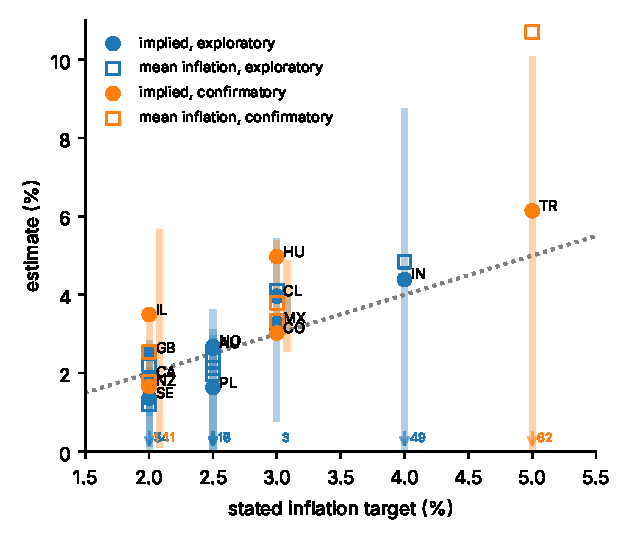
\includegraphics[width=0.6\textwidth]{fig_cb.pdf}
\caption{Implied inflation targets (filled) and mean inflation (open squares) against stated targets; vertical bars are 90\% bootstrap intervals over the bounded replicates (Table~\ref{tab:boot}); Turkey's is not drawn.}\label{fig:cb}\end{figure}

\paragraph{Uncertainty.} Table~\ref{tab:boot} reports 90\% moving-block bootstrap intervals (blocks of 8 quarters, 100 replicates per bank). Refitting with the full estimator takes several minutes per replicate, so the replicates use a lighter search (differential evolution with 800 generations and population 40, followed by the linear program, without the large-neighbourhood step). In some replicates the transmission parameter $\alpha$ reaches its lower bound, which makes $\tau=c/\alpha$ unbounded; we count these replicates separately and take quantiles over the others, so the intervals describe the bounded fits only. Degenerate replicates are frequent for the United Kingdom (42), Turkey (39), India (29) and Norway (10); the lighter search may contribute to this, and for these banks the target is less well determined than the point estimate suggests. Twelve of fourteen intervals contain the stated target; Mexico's (3.18--3.89) excludes 3\% narrowly and Poland's (0.66--2.18) excludes 2.5\%. The width separates reliable from unreliable estimates: intervals are about 1 pp wide for Australia, Canada, the United Kingdom and Mexico, but 4 pp or more for Chile and Israel, and Turkey's interval is unbounded below. Sweden's interval (0.21--2.15) only just reaches its 2\% target; its inflation averaged 1.2\% over the window. Covering the stated target is weak evidence where intervals are wide.
\begin{table}[t]\centering\small\begin{tabular}{lrrrrcr}\toprule
Bank & Stated & 5\% & Median & 95\% & \hd{Covers\\stated} & \hd{Degenerate\\replicates} \\\midrule
AU & 2.5 & 2.06 & 2.63 & 3.03 & yes & 0\\
CA & 2.0 & 1.31 & 1.89 & 2.27 & yes & 1\\
CL & 3.0 & 0.99 & 3.63 & 5.32 & yes & 0\\
CO & 3.0 & 2.69 & 3.06 & 4.65 & yes & 0\\
GB & 2.0 & 1.79 & 2.51 & 2.77 & yes & 42\\
HU & 3.0 & 2.90 & 4.10 & 5.23 & yes & 0\\
IL & 2.0 & 0.43 & 1.45 & 4.43 & yes & 4\\
IN & 4.0 & 2.38 & 4.70 & 6.27 & yes & 29\\
MX & 3.0 & 3.18 & 3.47 & 3.89 & no & 0\\
NO & 2.5 & 1.79 & 2.68 & 3.54 & yes & 10\\
NZ & 2.0 & 1.65 & 2.84 & 3.45 & yes & 0\\
PL & 2.5 & 0.66 & 1.56 & 2.18 & no & 8\\
SE & 2.0 & 0.21 & 0.88 & 2.15 & yes & 0\\
TR & 5.0 & -29.88 & 7.46 & 10.17 & yes & 39\\
\bottomrule\end{tabular}
\caption{Moving-block bootstrap of the implied inflation target (100 replicates, blocks of 8 quarters). Quantiles over replicates in which $\alpha$ is above its lower bound; last column: replicates with $\alpha$ at its bound ($\tau$ unbounded).}\label{tab:boot}\end{table}


\paragraph{Robustness.} The results depend on the inflation horizon (Table~\ref{tab:sens} in the Appendix, one search seed per fit). With inflation 2 or 6 quarters ahead instead of 4, three and two of fourteen fits are degenerate ($\alpha$ at its bound, $\tau$ unbounded); among the others, the mean absolute error is 0.80 and 0.93 pp against 1.02 and 0.42 for average inflation, and the implied target is closer than average inflation in four of seven and two of four off-target banks. Ending the sample in 2015 gives 0.75 against 0.48 and four of five off-target banks. The four-quarter horizon was fixed before the development results and pre-specified for the confirmatory test, but the advantage over average inflation is not robust to the horizon.

\paragraph{Search seeds.} We refitted every bank with five search seeds. The best of the five gives the reported target for twelve banks; for Hungary it finds a 2\% lower loss with target 3.90 instead of 4.97, and for Australia 2.76 instead of 2.63. For six banks (Chile, Hungary, Israel, India, Norway, Sweden) seeds whose losses lie within 9\% of the best give targets more than 0.5 pp apart, so these targets are not well determined. With the best of five seeds the mean absolute error over fourteen banks would be 0.58 pp (0.53 without Turkey) instead of 0.64 (0.61), still no better than a constant 2.5\% without Turkey, and the confirmatory criterion is unchanged (results/cb\_multiseed.csv). The lighter search used for the bootstrap below, run from the same five seeds, gives the same target (within 0.03) for eleven banks; for Israel it finds a 5\% lower loss with target 3.37, and for India and Norway nearly equal losses with targets 2.38 and 2.48 (results/cb\_light\_point.csv). Where targets differ across seeds with nearly equal loss, the loss surface is flat in $\tau$ and the reported value is one of several equally good fits.

\subsection{Official development assistance}\label{sec:aid}
We use OECD DAC1 donor totals: net ODA as a percentage of GNI on the net disbursement basis (1960--2017) and grant-equivalent ODA (from 2018); the change between 2017 and 2018 spans the definitional break and is dropped. The sample contains the 23 bilateral donors with at least 30 annual decisions (30--63 each). Each donor is estimated exactly with Theorem~\ref{thm:exact} (Table~\ref{tab:aid}). The 0.7\% of GNI target was adopted by the UN General Assembly in 1970 and accepted by most donors, though not all: the United States never accepted it \citep{clemens2007}, and some donors set themselves higher national goals.

Before interpreting a revealed target we ask two questions of each donor's decisions, with one test for each; $p$-values are adjusted across the 23 donors by the Benjamini--Hochberg procedure (BH).

\emph{Do decisions depend on the level at all?} The statistic is the in-sample gain of the fitted goal program over always holding, $1-\hat L/\overline{|D|}$. Under the null hypothesis decisions carry no information about the level: we permute the decisions, rebuild the level path from the first observation by $x_{t+1}=x_t+\Delta_t$ (keeping the jumps at the 2018 break), refit the exact estimator and recompute the gain ($B=999$ permutations). On 200 simulated series with independent decisions the test rejected in 2\% of cases at the 5\% level and in 7\% at the 10\% level. Rebuilding the level path matters: permuting decisions while keeping the observed levels rejected in 9\% of null series at the 5\% level, because observed levels already encode past decisions. Permutation also destroys any persistence in decisions, and persistence alone produces some rejections: with AR(1) decisions (coefficient 0.7) that do not depend on the level, the test rejected in 9\% of 100 series at the 5\% level (12\% at 10\%; Monte Carlo standard error about 3 points), and with a drift that switches regime at random in 8\% (13\%). The test therefore detects state dependence, not goal-seeking specifically, and is somewhat liberal under persistent decisions. After adjustment, seven donors show state dependence at the 10\% level (Sweden, Belgium, Portugal, France, Norway, Turkey, New Zealand) and four at 5\% (Sweden, Belgium, Portugal, France).

\emph{Is the goal program a better description than partial adjustment?} The second test takes linear partial adjustment, $\Delta_t=\mu+\kappa x_t+\varepsilon_t$, as the null. We fit it by least absolute deviations, simulate decisions by resampling its residuals, rebuild the level path as above, and compare the statistic $S=L_{\mathrm{PA}}/L_{\mathrm{GP}}$, the ratio of the in-sample mean absolute errors of the two fits, with its distribution over $B=999$ simulated series. Residuals are resampled either independently or in moving blocks of three years, which keeps short-run persistence. We checked the size on 60 simulated series of 60 decisions for each of four null behaviours (partial adjustment with independent or AR(1) errors, independent decisions, and AR(1) decisions unrelated to the level; 199 draws per series): rejection rates at the 5\% level were 0--7\% and at the 10\% level 0--17\%, against a Monte Carlo standard error of about 4 points. The power is modest: on series generated by a goal program with a band of width 0.3 and steps of 0.05 the test rejects in 16\% (independent residuals) and 12\% (blocks) of 100 series at 5\%, and on series from the rate-limited quadratic program of Section~\ref{sec:adequacy}, which is not a goal program, in 59\% and 62\% (results/pa\_null\_extend.csv). A rejection therefore shows that decisions respond to the level nonlinearly, with a dead zone or saturation that a linear rule cannot produce; it does not single out the goal program among nonlinear rules. After adjustment, partial adjustment is rejected at the 10\% level for Sweden, Norway, Portugal, Turkey, Japan and Luxembourg with independent residuals, and for the same donors except Luxembourg with block residuals.

\emph{Combining the two tests.} We call a donor's revealed target interpretable when both hypotheses are rejected, and control the false discovery rate of this conjunction by applying the Benjamini--Hochberg procedure to $\max(p_{\mathrm{state}},p_{\mathrm{PA}})$, which is valid for an intersection--union test. With independent residuals Sweden (adjusted 0.02), Portugal (0.06) and Norway (0.10) qualify at the 10\% level; with block residuals only Sweden does (0.07), and Portugal, Norway and Turkey follow at 0.13 (Table~\ref{tab:aid}). The evidence for goal-seeking aid behaviour is therefore strong for one donor and moderate for two; for the others the bands are descriptive. Decisions themselves are not persistent: the first-order autocorrelation of annual changes has median $-0.18$ across donors and exceeds 0.3 only for France and Turkey (results/aid\_autocorr.csv), so the liberal size of the permutation test under persistence (above) matters little here.

\emph{What the revealed targets say.} Sweden's revealed target is 0.90\% of GNI and Norway's 0.98\%, both well above their mean levels (0.77 and 0.80) and near their national 1\% goals; Portugal's is 0.27\%, close to its mean level (0.21). A revealed target close to the mean level is what a mean-reverting rule without a dead zone would also produce, so for low-level donors such as Portugal, Japan (0.28 against 0.25) and the United States (0.21 against 0.25) the target adds little to the average; Table~\ref{tab:aid} reports $\hat\tau$ minus the mean level for every donor. The large steps down for Sweden (0.43 pp) and Portugal (0.35) rest on single episodes: Sweden's largest cut while above its band was 0.46 pp and Portugal's 0.42, while all other cuts above the band were 0.23 pp or less, so the fitted step is the size of one large cut and smaller gaps are closed by moving to the band edge. Near-optimal sets are truncated at zero, which affects Australia, Germany, the United Kingdom and Turkey, whose sets are wide.

\emph{Goals.} Table~\ref{tab:aidgt} applies one rule to every donor in the sample with a documented goal: five national goals verified from OECD peer reviews and parliamentary documents after the estimates had first been produced, the United Kingdom's statutory 0.7\% (2015), and the 2005 commitment of the EU-15 members to reach 0.7\% by 2015. The question is whether the goal lies in the revealed band and in the near-optimal set. Of fifteen donors, the goal lies in the band for four (Norway, Luxembourg, Denmark, Germany) and in the set for six (also the Netherlands and the United Kingdom, whose set is nearly uninformative). Sweden's goal lies just above both. Of the nine donors scored against the EU-15 commitment, eight reveal targets well below 0.7\%, from 0.14 (Italy) to 0.59 (Finland), consistent with the commitment not having been met; Germany's band reaches 0.76 but its set is wide. The estimates use the whole period while the goals were adopted at different dates, and the comparison was not specified in advance.

\emph{Measuring the level.} The state is the previous year's share of GNI, so GNI growth moves it without any decision. Replacing it by the previous year's aid volume divided by this year's GNI (both in national currency; Turkey dropped, years with aid below 5 million excluded) changes the revealed target by a median of 0.05 pp across 22 donors, but by up to 0.43 (the United Kingdom, from 0.27 to 0.70). It moves the high-aid donors towards their national goals: Sweden to 0.98 (set 0.96--1.03, which contains 1\%), Norway to 1.05, Luxembourg to 1.01 and Denmark to 1.03 (last column of Table~\ref{tab:aidgt}; results/aid\_gni\_drift.csv). The main estimates should therefore be read as revealed targets for the share measured before GNI growth.
\begin{table}[t]\centering\footnotesize\setlength{\tabcolsep}{3pt}\begin{tabular}{llcccccc}\toprule
Donor & Goal & \hd{Revealed\\band} & \hd{$\tau$ set\\(2\%)} & \hd{Goal in\\band; set} & \hd{Mean\\level} & \hd{GNI-adjusted\\$\hat\tau$ (set)} & \hd{Both tests\\(BH)}\\\midrule
SWE & 1.0 (N, to 2022) & [0.83, 0.97] & (0.88, 0.95) & no; no & 0.77 & 0.98 (0.96, 1.03) & 0.02\\
NOR & 1.0 (N, 2005) & [0.93, 1.03] & (0.95, 1.05) & yes; yes & 0.80 & 1.05 (1.02, 1.25) & 0.10\\
LUX & 1.0 (N, 1999) & [1.00, 1.00] & (1.00, 1.01) & yes; yes & 0.63 & 1.01 (1.01, 1.04) & 0.22\\
DNK & 0.8 (N, 2011) & [0.71, 1.01] & (0.78, 0.87) & yes; yes & 0.70 & 1.03 (0.98, 1.13) & 0.32\\
NLD & 0.7 (N, 2012) & [0.49, 0.61] & (0.49, 0.73) & no; yes & 0.73 & 0.87 (0.79, 1.03) & 0.35\\
GBR & 0.7 (S, 2015) & [0.27, 0.27] & (0.00, 1.00) & no; yes & 0.43 & 0.70 (0.59, 0.82) & 0.99\\
AUT & 0.7 (EU, 2015) & [0.33, 0.35] & (0.26, 0.37) & no; no & 0.23 & 0.30 (0.26, 0.36) & 0.34\\
BEL & 0.7 (EU, 2015) & [0.46, 0.50] & (0.48, 0.50) & no; no & 0.48 & 0.51 (0.48, 0.52) & 0.35\\
DEU & 0.7 (EU, 2015) & [0.39, 0.76] & (0.00, 0.82) & yes; yes & 0.41 & 0.72 (0.52, 0.99) & 0.89\\
ESP & 0.7 (EU, 2015) & [0.10, 0.27] & (0.17, 0.28) & no; no & 0.22 & 0.25 (0.24, 0.35) & 0.68\\
FIN & 0.7 (EU, 2015) & [0.55, 0.64] & (0.49, 0.67) & no; no & 0.34 & 0.59 (0.53, 0.63) & 0.24\\
FRA & 0.7 (EU, 2015) & [0.44, 0.69] & (0.54, 0.59) & no; no & 0.55 & 0.63 (0.60, 1.36) & 0.26\\
IRL & 0.7 (EU, 2015) & [0.31, 0.55] & (0.35, 0.47) & no; no & 0.31 & 0.48 (0.46, 0.52) & 0.68\\
ITA & 0.7 (EU, 2015) & [0.13, 0.15] & (0.13, 0.28) & no; no & 0.20 & 0.26 (0.16, 0.36) & 0.99\\
PRT & 0.7 (EU, 2015) & [0.25, 0.28] & (0.23, 0.27) & no; no & 0.21 & 0.25 (0.24, 0.28) & 0.06\\
\bottomrule\end{tabular}
\caption{Revealed aid targets against documented goals (per cent of GNI), all donors in the sample with a goal. Goal: N national goal (year adopted; Sweden's held until 2022, the Netherlands' was about 0.8 before 2012), S statutory, EU the 2005 EU-15 commitment to reach 0.7\% by 2015. Near-optimal sets at 2\% tolerance from the exact profile loss, truncated at 0. GNI-adjusted: state measured as the previous year's aid volume over the current GNI. Last column: Benjamini--Hochberg adjusted $p$-value of the combined test (both hypotheses rejected; independent residuals). Sources and verification notes are in the supplementary material.}\label{tab:aidgt}\end{table}
\begin{table}[t]\centering\footnotesize\setlength{\tabcolsep}{3pt}\begin{tabular}{lrcccccc}\toprule
Donor & $n$ & \hd{State dependence\\$p$ (BH)} & \hd{GP vs PA\\$p$ (BH)} & $\hat\tau$ & \hd{Band\\($\tau$ set, 2\%)} & \hd{Steps\\(down, up)} & Mean\\\midrule
SWE$^{\dagger}$ & 63 & 0.001 (0.02) & 0.005 (0.04) & 0.90 & \hd{[0.83, 0.97]\\(0.88, 0.95)} & 0.43, 0.06 & 0.77\\
PRT$^{\dagger}$ & 43 & 0.005 (0.04) & 0.005 (0.04) & 0.27 & \hd{[0.25, 0.28]\\(0.23, 0.27)} & 0.35, 0.01 & 0.21\\
NOR$^{\dagger}$ & 63 & 0.013 (0.06) & 0.005 (0.04) & 0.98 & \hd{[0.93, 1.03]\\(0.95, 1.05)} & 0.08, 0.03 & 0.80\\
TUR$^{\dagger}$ & 30 & 0.022 (0.08) & 0.010 (0.05) & 0.56 & \hd{[0.56, 0.56]\\(-0.27, 0.58)} & 0.17, 0.01 & 0.25\\
LUX & 43 & 0.047 (0.11) & 0.010 (0.05) & 1.00 & \hd{[1.00, 1.00]\\(1.00, 1.01)} & 0.06, 0.03 & 0.63\\
JPN & 63 & 0.083 (0.15) & 0.015 (0.06) & 0.28 & \hd{[0.20, 0.37]\\(0.27, 0.31)} & 0.07, 0.06 & 0.25\\
FIN & 62 & 0.067 (0.14) & 0.025 (0.08) & 0.59 & \hd{[0.55, 0.64]\\(0.49, 0.67)} & 0.16, 0.01 & 0.34\\
USA & 63 & 0.079 (0.15) & 0.030 (0.09) & 0.21 & \hd{[0.19, 0.24]\\(0.21, 0.24)} & 0.03, 0.02 & 0.25\\
AUS & 63 & 0.238 (0.34) & 0.075 (0.19) & 0.49 & \hd{[0.43, 0.56]\\(-0.11, 0.58)} & 0.09, 0.00 & 0.39\\
CAN & 63 & 0.237 (0.34) & 0.095 (0.22) & 0.36 & \hd{[0.26, 0.47]\\(0.36, 0.38)} & 0.07, 0.02 & 0.35\\
DNK & 63 & 0.093 (0.15) & 0.120 (0.25) & 0.86 & \hd{[0.71, 1.01]\\(0.78, 0.87)} & 0.03, 0.02 & 0.70\\
FRA & 63 & 0.007 (0.04) & 0.145 (0.28) & 0.56 & \hd{[0.44, 0.69]\\(0.54, 0.59)} & 0.09, 0.01 & 0.55\\
AUT & 63 & 0.042 (0.11) & 0.190 (0.34) & 0.34 & \hd{[0.33, 0.35]\\(0.26, 0.37)} & 0.07, 0.02 & 0.23\\
NZL & 62 & 0.026 (0.09) & 0.205 (0.34) & 0.29 & \hd{[0.24, 0.34]\\(0.28, 0.33)} & 0.11, 0.01 & 0.26\\
BEL & 63 & 0.004 (0.04) & 0.235 (0.34) & 0.48 & \hd{[0.46, 0.50]\\(0.48, 0.50)} & 0.12, 0.04 & 0.48\\
NLD & 63 & 0.047 (0.11) & 0.235 (0.34) & 0.55 & \hd{[0.49, 0.61]\\(0.49, 0.73)} & 0.01, 0.07 & 0.73\\
ESP & 43 & 0.505 (0.61) & 0.445 (0.60) & 0.18 & \hd{[0.10, 0.27]\\(0.17, 0.28)} & 0.03, 0.04 & 0.22\\
CHE & 63 & 0.641 (0.74) & 0.535 (0.68) & 0.51 & \hd{[0.51, 0.51]\\(0.30, 0.58)} & 0.09, 0.01 & 0.30\\
IRL & 49 & 0.440 (0.60) & 0.570 (0.69) & 0.43 & \hd{[0.31, 0.55]\\(0.35, 0.47)} & 0.11, 0.01 & 0.31\\
DEU & 63 & 0.775 (0.85) & 0.665 (0.76) & 0.57 & \hd{[0.39, 0.76]\\(-0.04, 0.82)} & 0.03, 0.01 & 0.41\\
KOR & 36 & 0.958 (0.99) & 0.825 (0.90) & 0.15 & \hd{[0.15, 0.15]\\(0.15, 0.47)} & 0.00, 0.01 & 0.08\\
ITA & 63 & 0.473 (0.60) & 0.925 (0.93) & 0.14 & \hd{[0.13, 0.15]\\(0.13, 0.28)} & 0.02, 0.04 & 0.20\\
GBR & 63 & 0.986 (0.99) & 0.910 (0.93) & 0.27 & \hd{[0.27, 0.27]\\(-0.06, 1.00)} & 0.00, 0.03 & 0.43\\
\bottomrule\end{tabular}
\caption{Revealed ODA/GNI aspiration bands by donor (per cent of GNI). Columns 3--6: Benjamini--Hochberg adjusted $p$-values over the 23 donors of the state-dependence test (999 permutations), the test against partial adjustment with independent and block residuals (999 draws each), and the combined test on $\max(p_{\mathrm{state}},p_{\mathrm{PA}})$; raw values are in the supplementary material. $^{\dagger}$: combined adjusted $p$-value at most 0.10 with independent residuals. Sets truncated at 0. Bands of donors without evidence are descriptive.}\label{tab:aid}\end{table}
\begin{figure}[t]\centering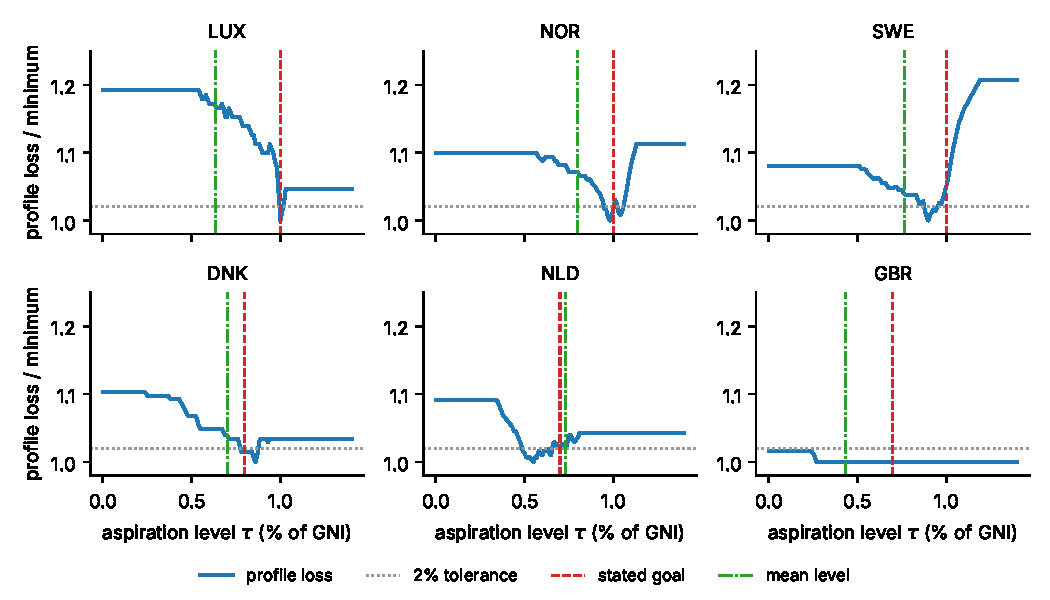
\includegraphics[width=\textwidth]{fig_aid_profiles.pdf}
\caption{Exact profile loss of the aspiration level for six donors, relative to its minimum. A sharp minimum indicates a well-determined target; the flat profile for the United Kingdom shows that its target is not determined.}\label{fig:aidprof}\end{figure}

\subsection{Defence spending}\label{sec:def}
We use NATO defence expenditure as a share of GDP (NATO definition, 31 allies, 2014--2025, the 2025 value an estimate; Finland and Sweden, which joined in 2023 and 2024, are included for all years, since NATO reports their spending from 2014) and pool allies with common parameters in two periods, before and after the 2022 invasion of Ukraine; the split is chosen by these events, not estimated. The state is the previous year's share and the decision its change. Table~\ref{tab:def} reports the estimates with two measures of uncertainty for the lower edge of the band: the set of lower edges whose exact profile loss is within 2\% of the optimum, and a 90\% cluster bootstrap interval that resamples allies with replacement (200 replicates), which respects the dependence of an ally's decisions over time.

In 2015--2021, 85\% of ally-years lie below the estimated band, and the fit says that allies below the band raised spending by about 0.03 points of GDP per year. The point estimate of the lower edge is 1.99\%, close to the 2\% guideline adopted in 2014 (Figure~\ref{fig:def}), but it is weakly determined: the bootstrap interval is 1.37--2.10, the profile loss is almost flat (2\% set 1.12--3.61), because a constant small increase fits most observations wherever the edge lies, and dropping one ally at a time moves it between 1.73 (without Romania) and 2.00. We therefore do not claim that the estimate recovers the 2\% guideline. In 2022--2025 the lower edge is 3.21\% and the step up 0.12 points per year (bootstrap 0.11--0.20, against 0.02--0.06 before). The two uncertainty measures disagree on whether the shift of the edge is distinguishable: the bootstrap intervals are disjoint (3.21--3.95 against 1.37--2.10), but the 2\% profile sets overlap (2.75--3.87 against 1.12--3.61), and the point estimate 3.21 is the lower limit of its own bootstrap interval, a sign that the edge is set by a few allies (dropping the United States moves it to 3.80). The rise in the step up is better determined than the rise in the edge. The upper edges and steps down rest on the 2\% of ally-years above the band and are not interpretable.

The decisions themselves give little evidence for the goal-program shape. We ran the two tests of Section~\ref{sec:aid} on the pooled panel: a permutation test that permutes decisions within each ally and rebuilds its spending path (999 permutations), and the test against linear partial adjustment with residuals resampled either independently or by ally (499 simulations). Neither rejects at the 5\% level in either period ($p$ between 0.08 and 0.82); out of sample, partial adjustment, holding and the median change all predict at least as well as the goal program (Table~\ref{tab:mcomp}). The defence estimates are therefore a description of how allies' spending changes varied with their level, not evidence that allies pursue a band. The shift is consistent with the move from the 2\% guideline towards the 3.5\% core target agreed in 2025, but the 2022 invasion changed the threat environment at the same time, and burden-sharing incentives within an alliance \citep{olson1966,sandler1995} also shape national spending; these cannot be separated here.
\begin{table}[t]\centering\small\begin{tabular}{lrcrrr}\toprule
Period & $n$ & Band & Step down & Step up & Mean level\\\midrule
2015-2021 & 217 & [1.99, 3.48] & 0.20 & 0.03 & 1.48\\
2022-2025 & 123 & [3.21, 3.66] & 0.21 & 0.12 & 1.85\\
\bottomrule\end{tabular}
\caption{Defence spending, pooled allies (per cent of GDP). The last two columns give the near-optimal set of the lower edge at 2\% tolerance (exact profile loss) and the 5--95\% range of the lower edge over 200 cluster-bootstrap replicates that resample allies.}\label{tab:def}\end{table}
\begin{figure}[t]\centering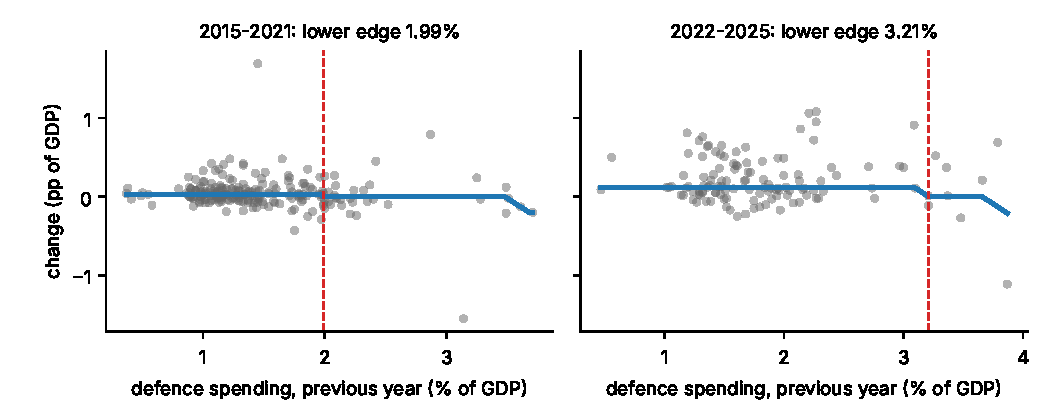
\includegraphics[width=\textwidth]{fig_defence.pdf}
\caption{Year-on-year changes in allies' defence spending against the previous level, with the fitted one-goal policy; the dashed line is the revealed lower edge of the band.}\label{fig:def}\end{figure}

\subsection{Corporate leverage}\label{sec:firms}
We use annual 10-K filings in the SEC Financial Statement Data Sets (2009--2026; firms with assets above USD 10 million), with book leverage, one minus equity over assets, as the goal variable. Its changes mix financing decisions with retained earnings and valuation changes, so the decision is measured with error. Firms are pooled by two-digit industry, with at most 3,000 randomly sampled firm-years per industry (Table~\ref{tab:firms}). The model is uninformative here: bands span most of the leverage range and step sizes are not identified. The one exception, depository institutions (SIC 60, band 0.87--1.00), is the industry whose capital is regulated (the Basel III leverage ratio sets a 3\% floor on Tier~1 capital relative to exposure; \citealp{bcbs2014}), but the regulatory floor would appear as the upper edge of the band, which is not determined, so the result does not test the regulation. A two-goal version that adds cash holdings did no better than predicting no change (results/firms\_k2.csv in the replication files).
\begin{table}[t]\centering\small\begin{tabular}{lrcrrr}\toprule
Industry & $n$ & Band & Step down & Step up & Mean level\\\midrule
SIC 13 & 1556 & [0.03, 0.83] & -- & -- & 0.47\\
SIC 28 & 3000 & [0.08, 0.82] & -- & -- & 0.37\\
SIC 35 & 1824 & [0.02, 0.93] & -- & 0.00 & 0.48\\
SIC 36 & 2930 & [0.02, 0.93] & -- & -- & 0.41\\
SIC 38 & 2812 & [0.07, 0.81] & -- & -- & 0.39\\
SIC 49 & 1543 & [0.03, 0.97] & -- & -- & 0.66\\
SIC 60 & 3000 & [0.87, 1.00] & -- & 0.01 & 0.89\\
SIC 63 & 1704 & [0.15, 0.98] & -- & -- & 0.75\\
SIC 67 & 3000 & [0.61, 1.23] & -- & 0.01 & 0.60\\
SIC 73 & 3000 & [0.08, 0.93] & 0.07 & 0.07 & 0.51\\
\bottomrule\end{tabular}
\caption{Book leverage, firms pooled by two-digit SIC industry; a dash marks a step that is not identified.}\label{tab:firms}\end{table}


\section{Model adequacy}\label{sec:adequacy}
The estimates are those of a goal program that rationalises the decisions (Theorem~\ref{thm:misspec}); an actor need not compute anything of the kind. Two questions follow: does the method invent targets when behaviour has no target, and is the goal program the best description of real decisions?

\paragraph{Placebo and misspecification experiments.} We simulated 100 series of 60 decisions from each of four behaviours (Table~\ref{tab:placebo}). In every case the state follows an AR(1) process with mean 2, coefficient 0.7 and innovation standard deviation 0.6, the decision is added to the state, and decisions carry Laplace noise with scale 0.03; seeds are fixed. The behaviours are an interval goal program (band $[1.5,2.5]$, steps 0.3 down and 0.4 up); random decisions drawn from $\{-0.3,0,0.4\}$ independently of the state (a coin flip); partial adjustment, $\Delta_t=0.3(2-x_t)$; and a quadratic program solved each period, $\min(x+\Delta-2)^2+2\Delta^2$ subject to $|\Delta|\le0.35$. On average the diagnostics separate random behaviour from goal-seeking: the fitted goal program improves on always holding by only 3\% in-sample, the near-optimal set of $\tau$ is 3.5 units wide, the estimates vary widely across replications, and out of sample the goal program beats holding in only 17\% of series. The raw diagnostics are not calibrated, however. The in-sample gain over holding is non-negative by construction, and 10\% of the random series yield a near-optimal set narrower than one unit, that is, a target that looks well determined. This share depends on the sample size more than on the noise: over noise scales 0.03, 0.1 and 0.2 it is 31--45\% at $T=30$, 10--14\% at $T=60$ and 1--5\% at $T=120$, while for the goal-program behaviour the set is narrower than one unit in at least 96\% of series in every cell, and its target error falls from 0.01--0.13 at $T=30$ to 0.004--0.03 at $T=120$ (results/placebo\_grid.csv). This is why the aid application relies on two calibrated tests (Section~\ref{sec:aid}): a permutation test of state dependence, whose size was checked on such series and under persistent decisions, and a parametric test against partial adjustment. For the other goal-seeking behaviours the revealed target is close to the reference level (1.99 for both), but partial adjustment predicts decisions better out of sample in 95--100\% of series, so model comparison identifies the misspecification. When the goal program is the true behaviour it beats partial adjustment in every series.
\begin{table}[t]\centering\small\begin{tabular}{lrrrrrr}\toprule
True behaviour & $\hat\tau$ median & $\hat\tau$ IQR & Gain over hold & $\tau$-set width & GP beats hold & GP beats PA\\\midrule
Interval goal program & 2.00 & 0.01 & 78\% & 0.02 & 100\% & 100\%\\
Random (coin flip) & 2.05 & 0.83 & 3\% & 3.54 & 17\% & 25\%\\
Partial adjustment & 1.99 & 0.10 & 66\% & 0.06 & 100\% & 0\%\\
Quadratic program (solver) & 1.99 & 0.07 & 71\% & 0.06 & 100\% & 5\%\\
\bottomrule\end{tabular}
\caption{Placebo and misspecification experiments (100 replications each; PA: linear partial adjustment fitted by least absolute deviations; out-of-sample comparisons on the last 30\% of each series).}\label{tab:placebo}\end{table}

\paragraph{Real data.} Table~\ref{tab:mcomp} compares out-of-sample mean absolute errors of decisions (aid and central banks: last 30\% of each series; defence: five-fold cross-validation over allies). The goal program does not predict decisions better than simple rules: always holding has the lowest average error for aid and central banks, the goal program has strictly the lowest error for only 5 of 23 donors and 1 of 14 banks (Mexico), and it is worse than holding for 12 donors and 11 banks. These comparisons are imprecise: test windows are short (9--19 decisions per donor and 10--32 per bank), the bank models are fitted by the heuristic rather than the exact algorithm, and defence uses a single cross-validation over allies. Paired tests over units (sign test and Wilcoxon signed-rank on the per-unit errors, results/paired\_tests.csv) find no significant difference between the goal program and any rule for aid (smallest $p=0.06$, Wilcoxon against holding); for central banks the goal program is significantly worse than holding and than the median change (holding has the smaller error in 11 of the 12 banks without ties, sign test $p=0.006$, Wilcoxon $p=0.003$) and not distinguishable from the difference Taylor rule ($p=0.34$). Decisions are small and noisy relative to their variation, and aims change over time (Sweden left its 1\% goal in 2023; the Netherlands lowered its goal from about 0.8\% to 0.7\% in 2012), which a model with fixed parameters cannot anticipate. We therefore do not claim that interval goal programs are the best predictive model of these decisions. The claims of the paper concern the recovered aspiration levels. On that question the implied target of partial adjustment, $-\hat\mu/\hat\kappa$, is an alternative; it is undefined (no mean reversion) for five donors (Switzerland, Germany, Finland, the United Kingdom, Korea). For the five donors with verified national goals the revealed target is closer to the goal in three cases: Luxembourg (1.00 against 1.87, goal 1.0), Sweden (0.90 against 0.75, goal 1.0) and Denmark (0.86 against 1.41, goal 0.8), similar for Norway (0.98 against 1.01) and further for the Netherlands (0.55 against 0.75, goal 0.7). With five donors this is an illustration, not a test.
\begin{table}[t]\centering\small\begin{tabular}{lrrrrrrr}\toprule
Domain & Units & GP & PA & Hold & \hd{Median\\change} & \hd{GP strictly\\best} & \hd{GP worse\\than hold}\\\midrule
Aid (donors) & 23 & 0.056 & 0.052 & 0.049 & 0.050 & 5/23 & 12/23\\
Central banks & 14 & 0.481 & 0.413 & 0.380 & 0.380 & 1/14 & 11/14\\
Defence (periods) & 2 & 0.183 & 0.176 & 0.191 & 0.170 & 0/2 & 1/2\\
\bottomrule\end{tabular}
\caption{Out-of-sample mean absolute decision error of the goal program (GP), linear partial adjustment or difference Taylor rule (PA), always holding, and the median change; last column: number of units for which GP has the lowest error.}\label{tab:mcomp}\end{table}

\section{Discussion and conclusion}\label{sec:disc}
\paragraph{What the method adds.} Revealed aspiration levels are most informative when outcomes and announcements diverge. Average outcomes estimate the target well when an actor hits it; they say nothing about what an actor that misses is aiming for. For central banks the implied targets have the right magnitude and are much closer than average inflation where inflation and target diverged strongly (Turkey), but over all fourteen banks they are no closer to the stated target than a constant 2.5\%, so the stated targets offer only a weak check. In the aid application, the donors with the clearest evidence (Sweden, and less clearly Norway and Portugal) reveal targets of about 0.9--1.0\% of GNI (Sweden, Norway) and 0.27\% (Portugal), and most EU donors reveal targets well below their 0.7\% commitment; for low-level donors the revealed target is close to the mean level and adds little to it. For defence, the revealed lower edge rose from about 2\% to 3.2\% after 2022; the bootstrap separates the two periods but the profile loss does not, and no test distinguishes the decisions from simpler behaviour, so this result is descriptive.
\paragraph{When to trust an estimate.} The identification results say what the data must contain: periods in which a decision stops at a band edge for aspiration levels, and periods in which a single goal is outside its band for weights. Theorem~\ref{thm:cons} adds a support condition: the states must visit every regime of the policy, including both sides of the band. In the defence data only about 2\% of ally-years lie above the band, so the upper edge and the step down are weakly determined; this is the empirical face of the support condition failing. For aid the condition is better met (22\% of donor-years above and 44\% below the band), but donors whose shares hardly move, such as the United Kingdom, give flat profiles. In practice the exact profile loss for one goal and the bootstrap for several goals reveal when these conditions fail; the United Kingdom's aid series and the bootstrap intervals of several central banks are examples where the method itself reports that the target is not determined.
\paragraph{Limitations.} The goal program is not a better predictor of decisions than simple rules (Section~\ref{sec:adequacy}). The central-bank results are sensitive to the inflation horizon (Section~\ref{sec:cb}). The forward model is myopic and linear in transmission; central banks plan over horizons and face uncertain transmission. Inputs are proxies: realised inflation stands in for forecasts, and official forecasts are conditional on policy paths and drift to the target by construction. The confirmatory sample is small and the confirmatory criterion was met in only three banks. The test of state dependence is somewhat liberal under persistent decisions, and the test against partial adjustment has modest power against a goal program and also rejects other nonlinear rules. The aid state is a share of GNI, which GNI growth moves without any decision. Pooling allies imposes common parameters, and the 2022 invasion of Ukraine coincides with the change in NATO guidance. Revealed aspiration levels are those of a goal program that rationalises the decisions; they are not a claim about the decision maker's reasoning, and political economy can masquerade as preferences.
\paragraph{Extensions.} Forward-looking (multi-period) goal programs, an exact algorithm with a certificate for several goals, heterogeneous actors with shared structure (clustering in the spirit of \citet{carrizosa2026}), and statistical rates and confidence sets for the identified set are natural next steps.

\paragraph{Conclusion.} Inverse interval goal programming turns a sequence of decisions into aspiration levels, tolerance bands and step sizes. The structure of goal programs makes the problem tractable and its identification transparent. In public data the revealed aspirations are of the right magnitude where targets are known and differ across actors that share a commitment; how much the data say about them must be checked case by case, with the profile loss, the bootstrap and tests against simpler rules.

\section*{Declarations}
\begin{itemize}
\item Funding: No funding was received for conducting this study.
\item Competing interests: The author has no competing interests to declare that are relevant to the content of this article.
\item Ethics approval and consent to participate: Not applicable; the study uses only published aggregate data.
\item Data availability: All data are publicly available from the Bank for International Settlements, the OECD, Eurostat, NATO, the World Bank and SEC EDGAR; download scripts are provided with the code.
\item Code availability: The code and data that reproduce all tables and figures are available at \url{https://github.com/vinhqdang/Multiple-Objective-Programming-and-Goal-Programming}.
\item Author contribution: The sole author designed the study, carried out the analysis and wrote the manuscript.
\end{itemize}


\begin{appendices}
\section{Specifications tried during development}\label{app:specs}
For transparency, Table~\ref{tab:specs} lists the central-bank specifications estimated before the gradualism model, in the order they were run.
\begin{table}[h]\centering\small
\begin{tabular}{p{6.8cm}rr}\toprule
Specification & \hd{MAE\\implied} & \hd{MAE mean\\inflation}\\\midrule
Sign-only interval rule, current inflation (linear program) & 0.46 & 0.48\\
Linear cost, $K=1$, current inflation, exact MILP & 0.94 & 0.47\\
Linear cost, $K=2$, inflation 4 quarters ahead and growth gap, MILP & 0.72 & 0.47\\
Linear cost, $K=2$, hybrid search & 1.55 & 0.47\\
Linear cost, $K=2$, official forecasts (5 banks) & 1.83 & 0.22\\
Quadratic cost (gradualism), $K=2$, realised inputs (reported) & 0.45 & 0.47\\
\bottomrule\end{tabular}
\caption{Central-bank specifications in order of estimation (nine exploratory banks unless stated).}\label{tab:specs}\end{table}

\section{Sensitivity of the implied inflation targets}\label{app:sens}
\begin{table}[h]\centering\small\begin{tabular}{lrrrrr}\toprule
Bank & Stated & 4 quarters (main) & 2 quarters & 6 quarters & End 2015\\\midrule
AU & 2.5 & 2.63 & 1.47 & 2.79 & 2.63\\
CA & 2.0 & 1.89 & deg. & 2.38 & 1.89\\
CL & 3.0 & 3.96 & 3.91 & 1.38 & 4.84\\
CO & 3.0 & 3.02 & 4.25 & 2.73 & 2.82\\
GB & 2.0 & 2.51 & deg. & 2.51 & 2.51\\
HU & 3.0 & 4.97 & 3.16 & 3.93 & 4.97\\
IL & 2.0 & 3.49 & 2.66 & 5.26 & 1.04\\
IN & 4.0 & 4.39 & 3.46 & deg. & --\\
MX & 3.0 & 3.27 & 3.53 & 3.23 & 3.69\\
NO & 2.5 & 2.68 & 1.69 & 1.77 & 3.19\\
NZ & 2.0 & 1.66 & deg. & 2.58 & 1.66\\
PL & 2.5 & 1.63 & 1.74 & 1.97 & 1.56\\
SE & 2.0 & 1.36 & 0.98 & 0.10 & 1.36\\
TR & 5.0 & 6.14 & 6.14 & deg. & --\\
\bottomrule\end{tabular}
\caption{Implied inflation targets under alternative inflation horizons and sample ends (gradualism model, realised inputs; ``deg.'' marks a degenerate fit with $|\hat\tau|>15$; ``--'' too few quarters).}\label{tab:sens}\end{table}

\end{appendices}

\bibliography{refs}
\end{document}
